\subsection{Nomenclature}

As detailed earlier, many experiments have been run with varying configurations of the vehicle. Therefore, in this section, for clarity, the configurations will be referred to according to Table 1.

% Please add the following required packages to your document preamble:
% \usepackage[table,xcdraw]{xcolor}
% If you use beamer only pass "xcolor=table" option, i.e. \documentclass[xcolor=table]{beamer}
\begin{table}[H]
\caption{Experimental setup configurations. "D" for disconnected, "C" for connected}
\label{tab:experimentConfigs}
\centering
\begin{tabular}{|
>{\columncolor[HTML]{\CellColor}}l |l|l|l|}
\hline
\textbf{Configuration name} & \cellcolor[HTML]{\CellColor}\textbf{Gearbox} & \cellcolor[HTML]{\CellColor}\textbf{Chain} & \cellcolor[HTML]{\CellColor}\textbf{Propeller} \\ \hline
\textbf{(A)}                & D                                        & D                                      & D                                          \\ \hline
\textbf{(B)}                & C                                        & D                                      & D                                          \\ \hline
\textbf{(C)}                & C                                        & C                                      & D                                          \\ \hline
\textbf{(D)}                & C                                        & C                                      & C                                          \\ \hline
\end{tabular}
\end{table}

\subsection{Drivetrain performance}

\begin{figure}
    \centering
    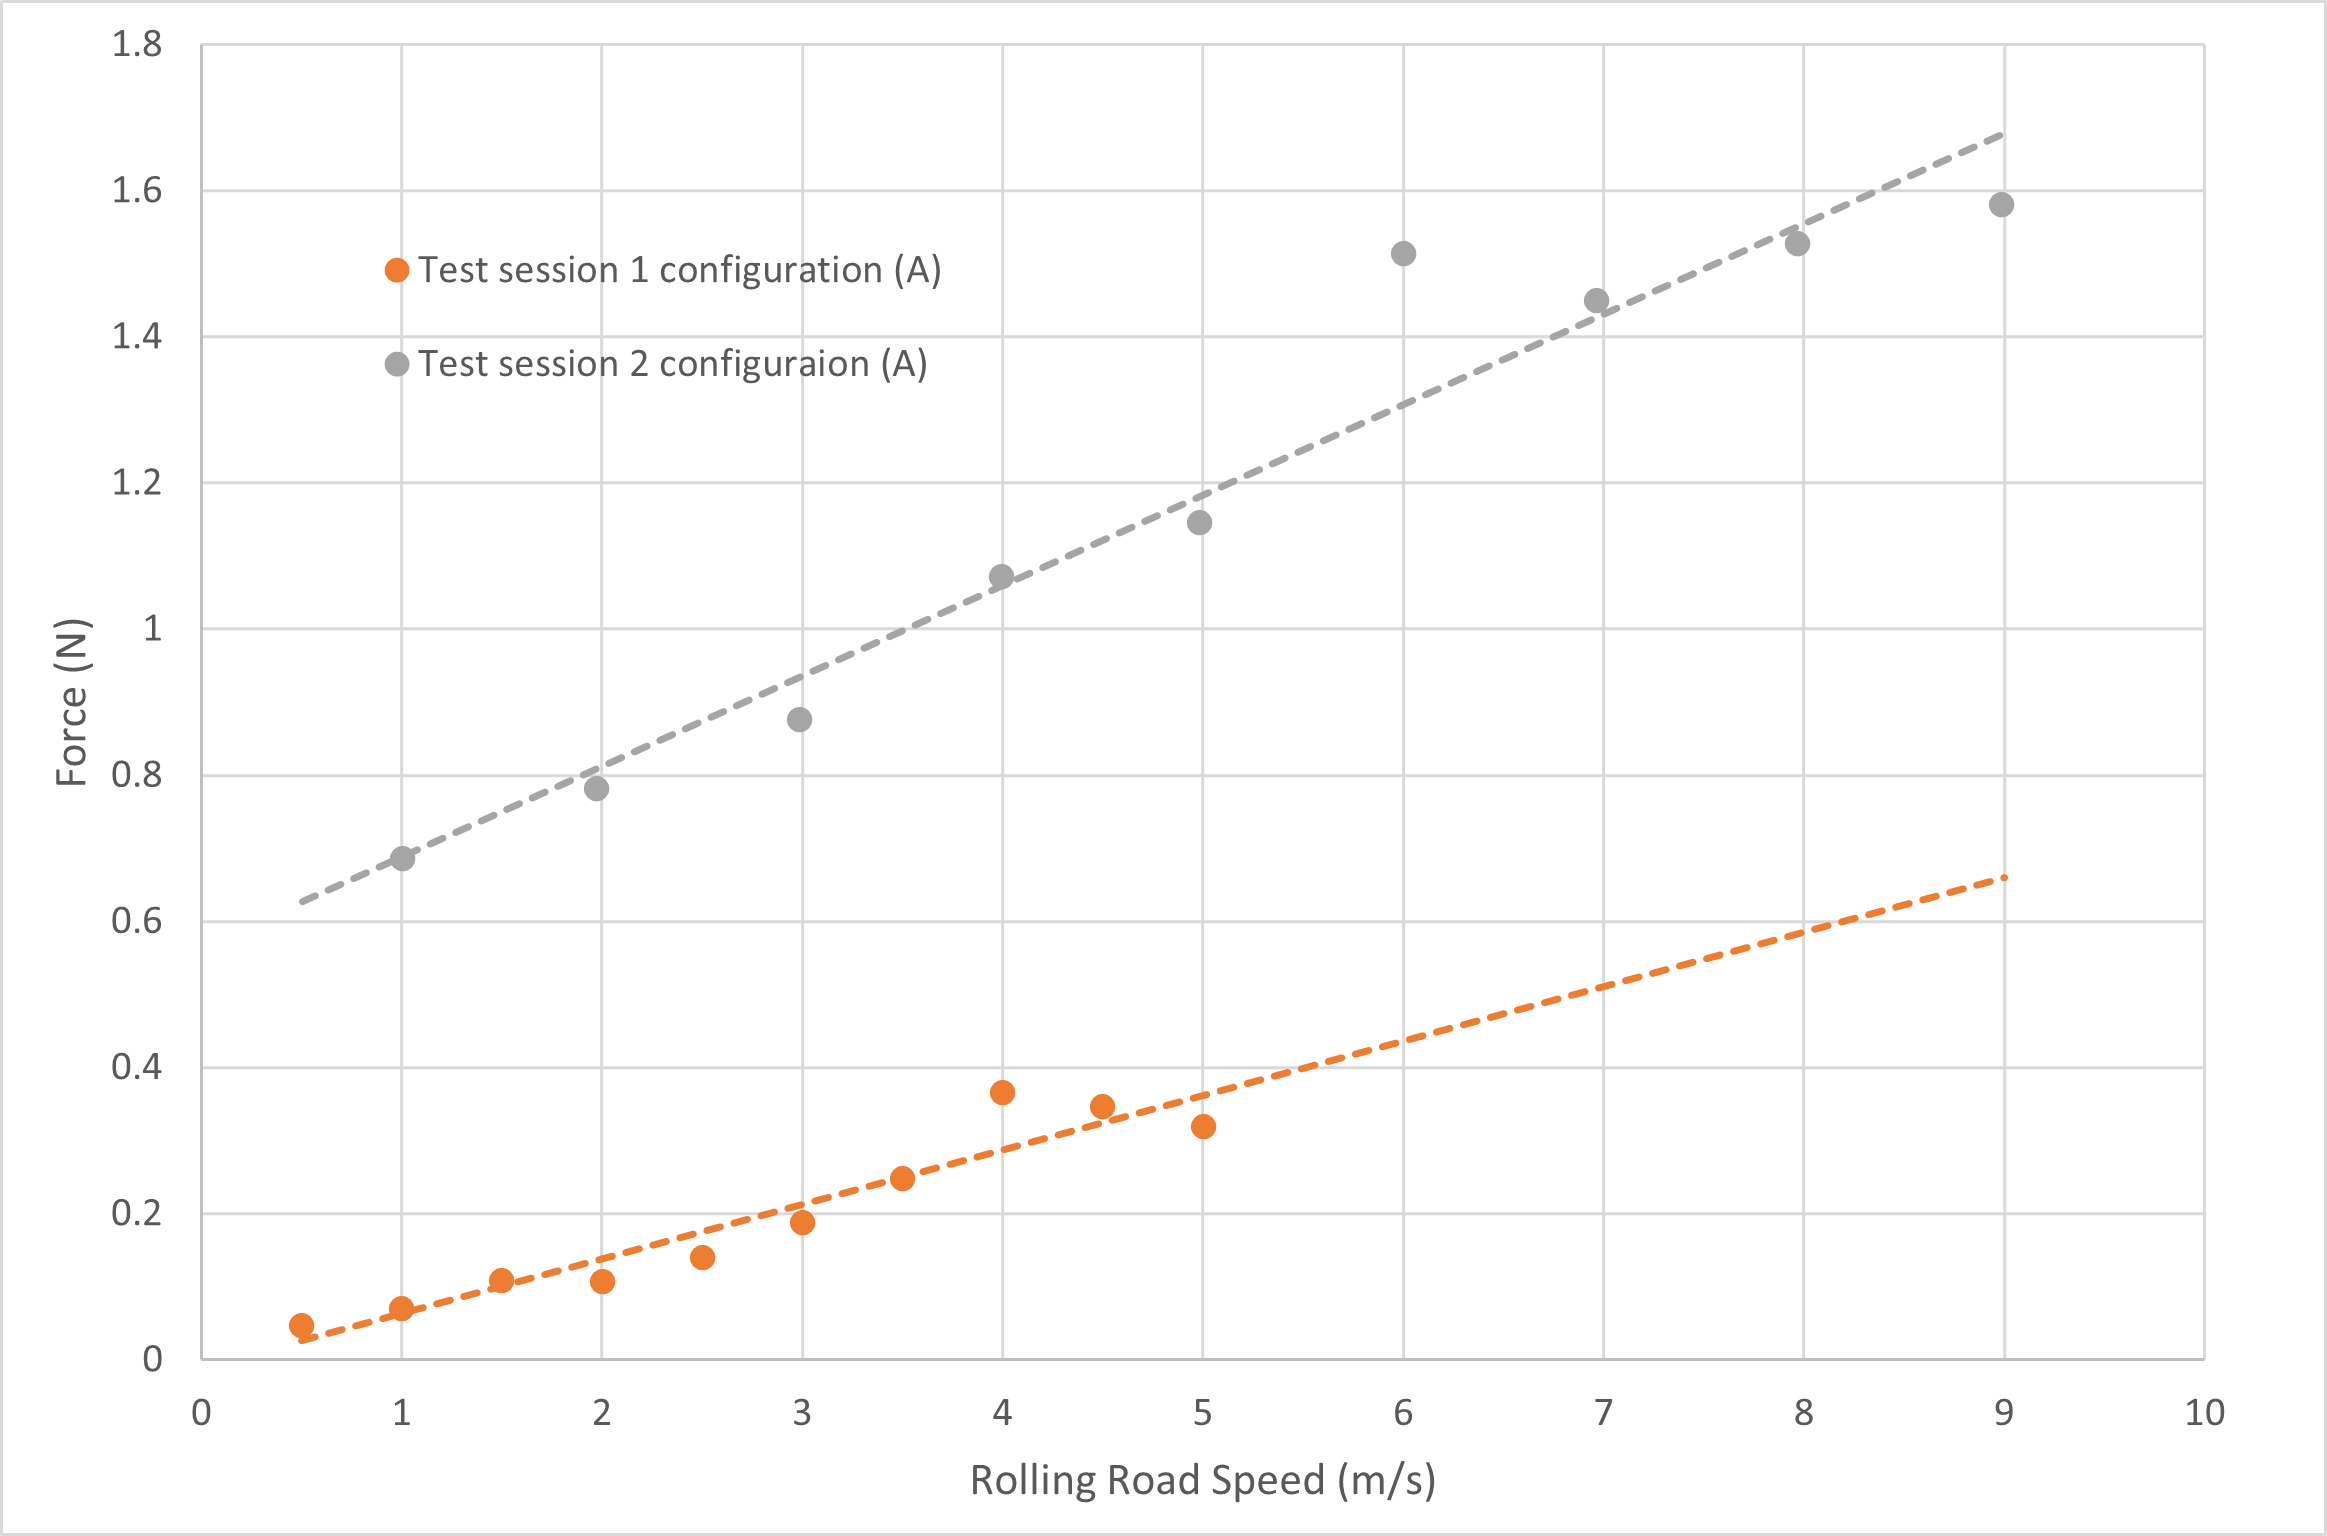
\includegraphics[width = 0.7\linewidth]{images/part11/zeroingcomparison.png}
    \caption{Total force on the vehicle as a function of the rolling road speed for the different test sessions - Baseline experimental setup.}
    \label{fig:zeroing}
\end{figure}

Figure \ref{fig:zeroing} illustrates a discrepancy between the first and the second set of results from each session. The measurements taken in the second test, represented here by the grey dataset, displayed a higher force overall than the corresponding measurements of the first session. Although the vehicle had gone through structural changes, it was hypothesised that zeroing issues during the first tests could be the cause. Indeed, the forces measured tend towards zero as the road speed approaches zero is not consistent with what would be expected, where a minimum force would be required to move the vehicle from a stationary state. As a response to this, during the second test session, the zeroing process was completed by running the vehicle for 5 seconds at 0.5 m/s and then stopping. By completing the same process before each test, the data was more in line with expectations. In the first test, this was not completed as accurately, leading to offset results.

The chain tensioner was adjusted to a high tension to avoid the chain coming off. This also conveniently impacted the chain efficiency positively as shown in \cite{spicer2001effects}, where higher chain tension improves performance. The PLA used in the tensioner heated up and softened, causing the tension to suddenly reduce and the chain to come off. To avoid this, a short-term solution was proposed which meant the roller sprocket did not run as freely as desired, adding a large resistance to the chain drive. 

From the various results datasets, it is possible to notice a discontinuity in the results. This occurred at the same speed range in each case: 5 to 6 m/s. case, the increase in rearwards force was more significant than the resultant increase for speeds at either side of this section. Visually this was due to the vibrations in the structure of the vehicle inducing a horizontal force on the vehicle. The instantaneous fluctuation would cause significant oscillation in the chain which would potentially vary the force distribution on the propeller shaft during the operation. This behaviour is to be expected and follows patterns seen by \cite{conwell1992experimental} which stated that the dynamic effects of a chain are more apparent at higher ground speeds. The increased oscillation from the wheels would induce further dynamic effects on the chain and cause significant losses. This increase in dynamic effects could be seen to further increase the force on the drivetrain and therefore the losses seen in the vehicle.

Under quasi-static chain conditions, the dynamic effects on the chain can be neglected \cite{conwell1992experimental}. In this case’s chain system, this is apparent to be not true as the significant oscillation from the vehicle oscillation would increase these effects significantly and reduce the transmission of power for the vehicle.

The additional relation of the bearing effect on the drivetrain system increases the losses seen further. The top bearings of the system were very stiff and therefore would have a higher frictional coefficient than most general bearings. This increased stiffness was found by spinning the bearings independently. For bearing operation the frictional losses at higher RPM values tend to decrease approaching the quasi-static state of operation. 

The decrease in bearing frictional losses increases the efficiency of the prop shaft and chain system, ultimately reducing the overall contribution of the drivetrain to the losses. An investigation conducted by \cite{hammami2018friction} demonstrated the effects of different fluids and the effects on the frictional coefficient on a rolling bearing.

The behaviour of the bearings can be seen to affect the proportional losses of the system for both drivetrain setups. Both results show slight increases in efficiency over the range of the results which speculatively could be down to the bearing frictional losses reducing due to a more operational range being seen.

\begin{figure}[!htbp]
    \centering
    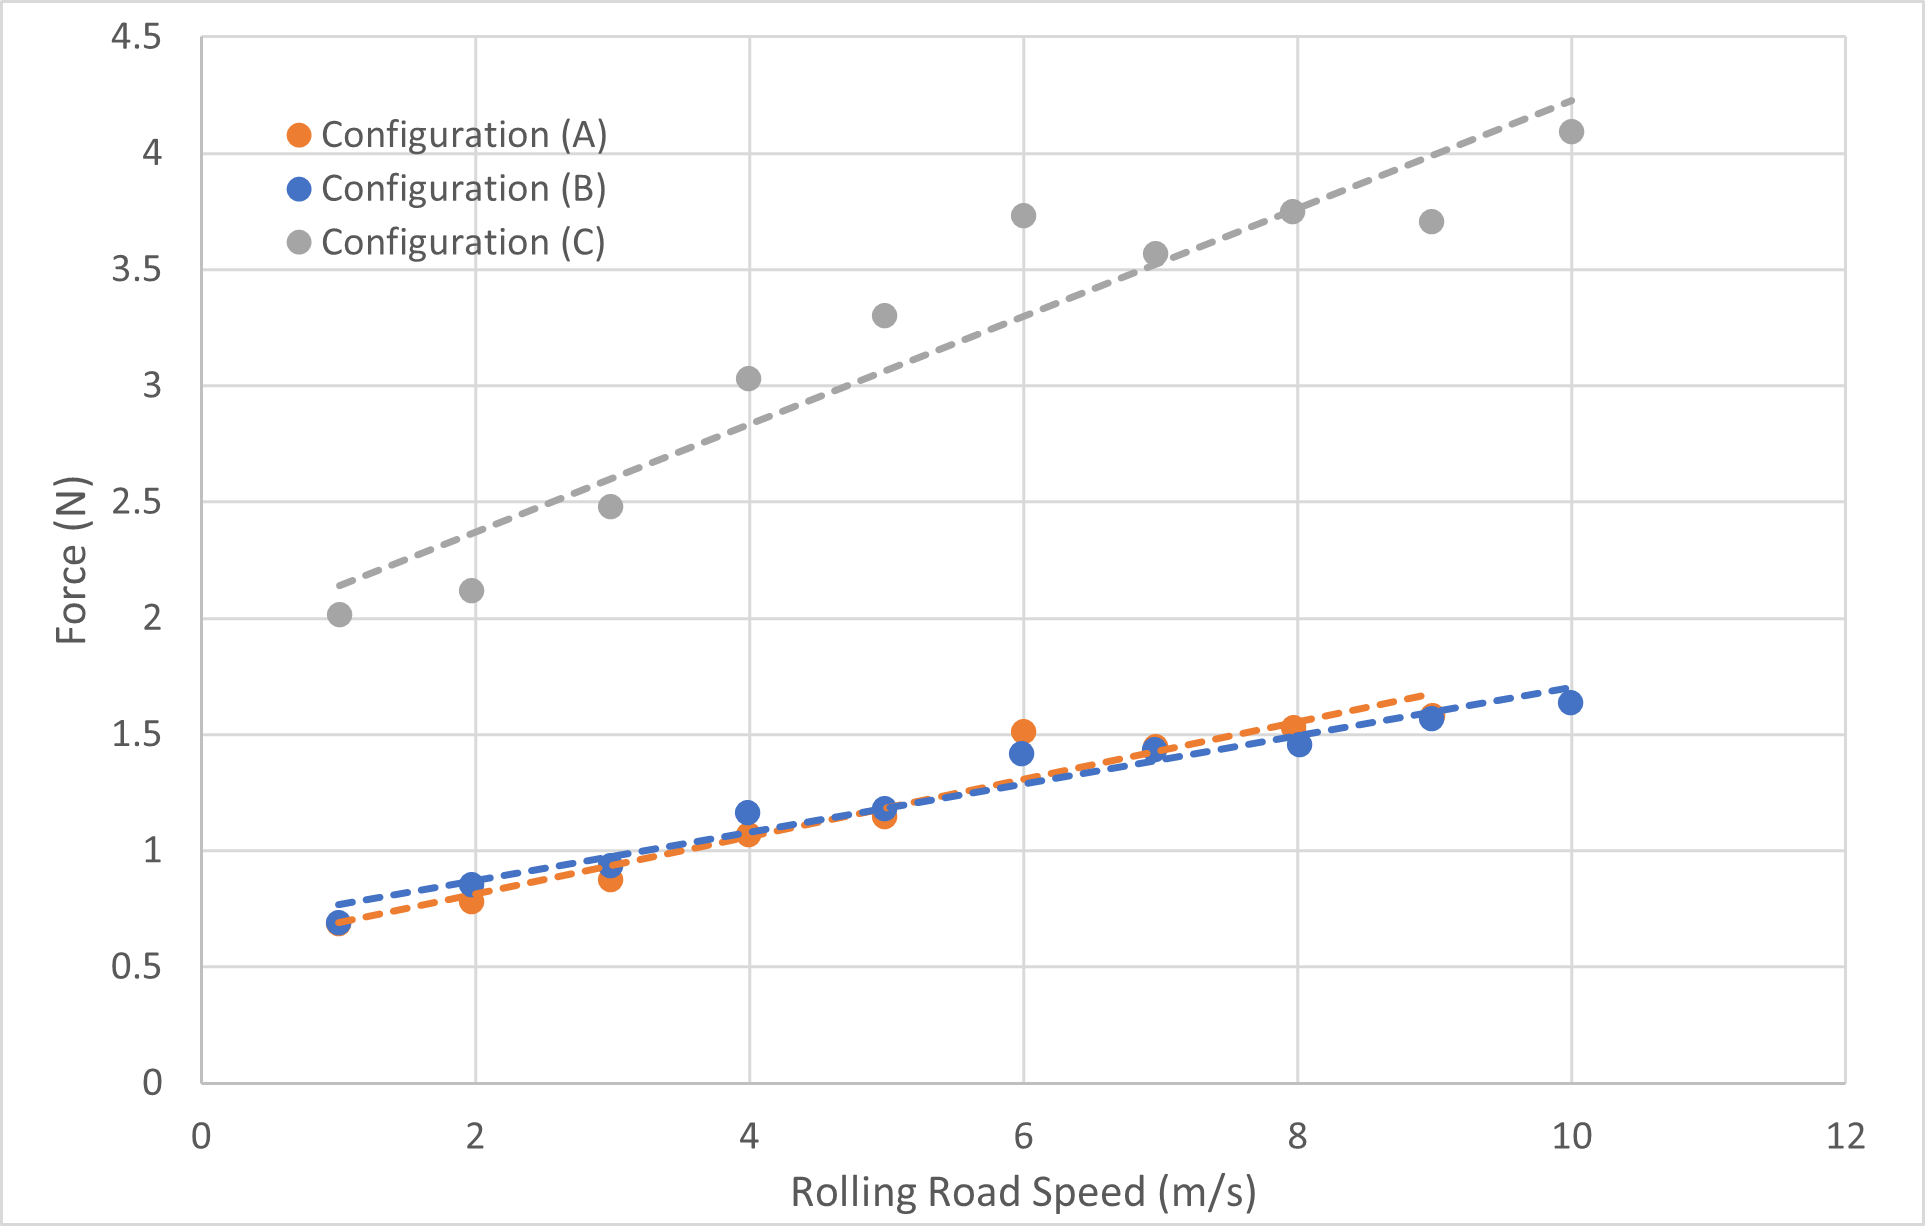
\includegraphics{images/part11/rollingresistancecomparisons.png}
    \caption{Total force on the vehicle as a function of speed for various configurations. Data from test session 2 - Baseline experimental setup.}
    \label{fig:rrsynthesis}
\end{figure}

For the second wind tunnel test day, an increase in percentage loss was seen for the chain system. The percentage loss over the range of rolling road speeds remains relatively constant which demonstrates the losses in the chain. There is a slight increase in losses at higher rolling ground speeds, but this could be down to the increased rolling resistance value contributing to loss in the system. The main finding from the second test is that the chain efficiency did reduce, which demonstrates the effect of the chain oscillating in the horizontal axis. At higher speeds, the oscillation on the chain did increase which would further describe the increase in negative force at these values. Figure \ref{fig:rr} demonstrates that the chain was the main location for losses in the drivetrain with significant losses being seen.

Figure \ref{fig:rrsynthesis} displays a direct comparison of the final vehicle tested in different configurations. The configurations without and with gearbox, (A) and (B) respectively, showed a negligible difference. The variance can be attributed to the standard deviation of the data being collected. The main difference is seen when the chain is connected to the system with the added losses from it and rolling resistance from the propeller shaft bearings contributing to almost a doubling in drag force on the vehicle. As is expected, the increase in rolling road speed causes an increase in the force due to friction. The results shown Figure \ref{fig:rrsynthesis} are comparable with each other as the zeroing process completed was the same for each example.


\begin{figure}[!htbp]
    \centering
    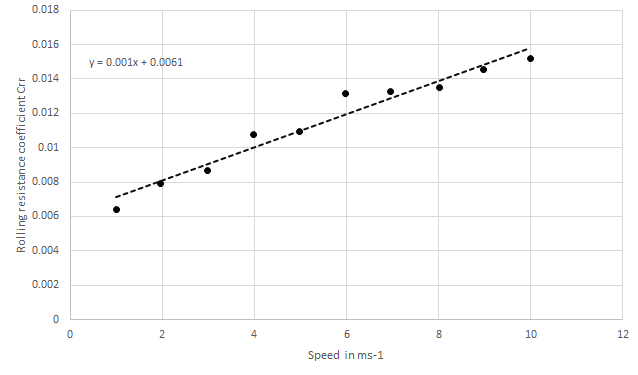
\includegraphics[width=0.9\linewidth]{images/part11/rollingresistance.png}
    \caption{Rolling resistance value from the wind tunnel data for session 2 - Baseline experimental setup.}
    \label{fig:rr}
\end{figure}

Figure \ref{fig:rr} demonstrates the rolling resistance of the vehicle in the second wind tunnel test day. Taking the rolling resistance results from the vehicle in configuration (A) (Figure \ref{fig:rrsynthesis}) and sharing the force values with the vehicle weight of 11 kg the vehicle rolling resistance coefficient was calculated. From interpolation, it can be seen that at 0 m/s the coefficient of rolling resistance is around 0.006 which according to Engineering toolbox \cite{rolling} is similar to the values expected for a truck tire, thus demonstrating the inefficiencies of the vehicle when rolling.

\subsection{Propeller performance assessment}

Figure \ref{fig:individualresults} shows the relevant results for propeller performance assessment. The top left and top right show the result of the baseline setup for configuration (D) and minimum and medium pitch respectively. The second row displays the same experimental setup for configurations (C) and (D) with maximum pitch. As mentioned in the data acquisition section, several short recordings were acquired for each point to obtain the standard deviation. The trendlines plotted on the graphs of Figure \ref{fig:individualresults} were added solely as a visual aid and do not rely on analytical trends.  

As seen comparing the different configurations in Figure \ref{fig:individualresults}, the minimum pitch case showed the least predictable behaviour as road speed increased. The reason for jump seen in the top left figure is unclear and may be due to the experimental conditions with the discontinuity in data points occurring at 5 m/s. This speed was observed to be a phase of instability for the vehicle. This is also shown on the other configurations, where the error bars are far greater for 5 m/s and its surroundings than for other speeds. 
 
Looking at Figure \ref{fig:individualresults} for the medium and maximum pitch cases, a clear decrease in the total force on the vehicle measured by the load cells showed a non-negligible contribution of the propeller. The total measured force remaining positive throughout the range implied that the vehicle would have been slower than the wind over the tested speed range. However, extrapolating using a quadratic fit curve on Figure \ref{fig:trendlineplot} indicated that better performance could have been achieved operating in wind faster than 10 m/s. It was modelled as a second order polynomial since propeller thrust increased quadratically with RPM (Figure \ref{fig:d}) and the rolling resistance seemed to increase linearly in this case over the studied speed range (Figure \ref{fig:rrsynthesis}). In this case, the quadratic coefficient is negative, which is simply due to the drag being taken as positive.

\begin{figure}
    \centering
    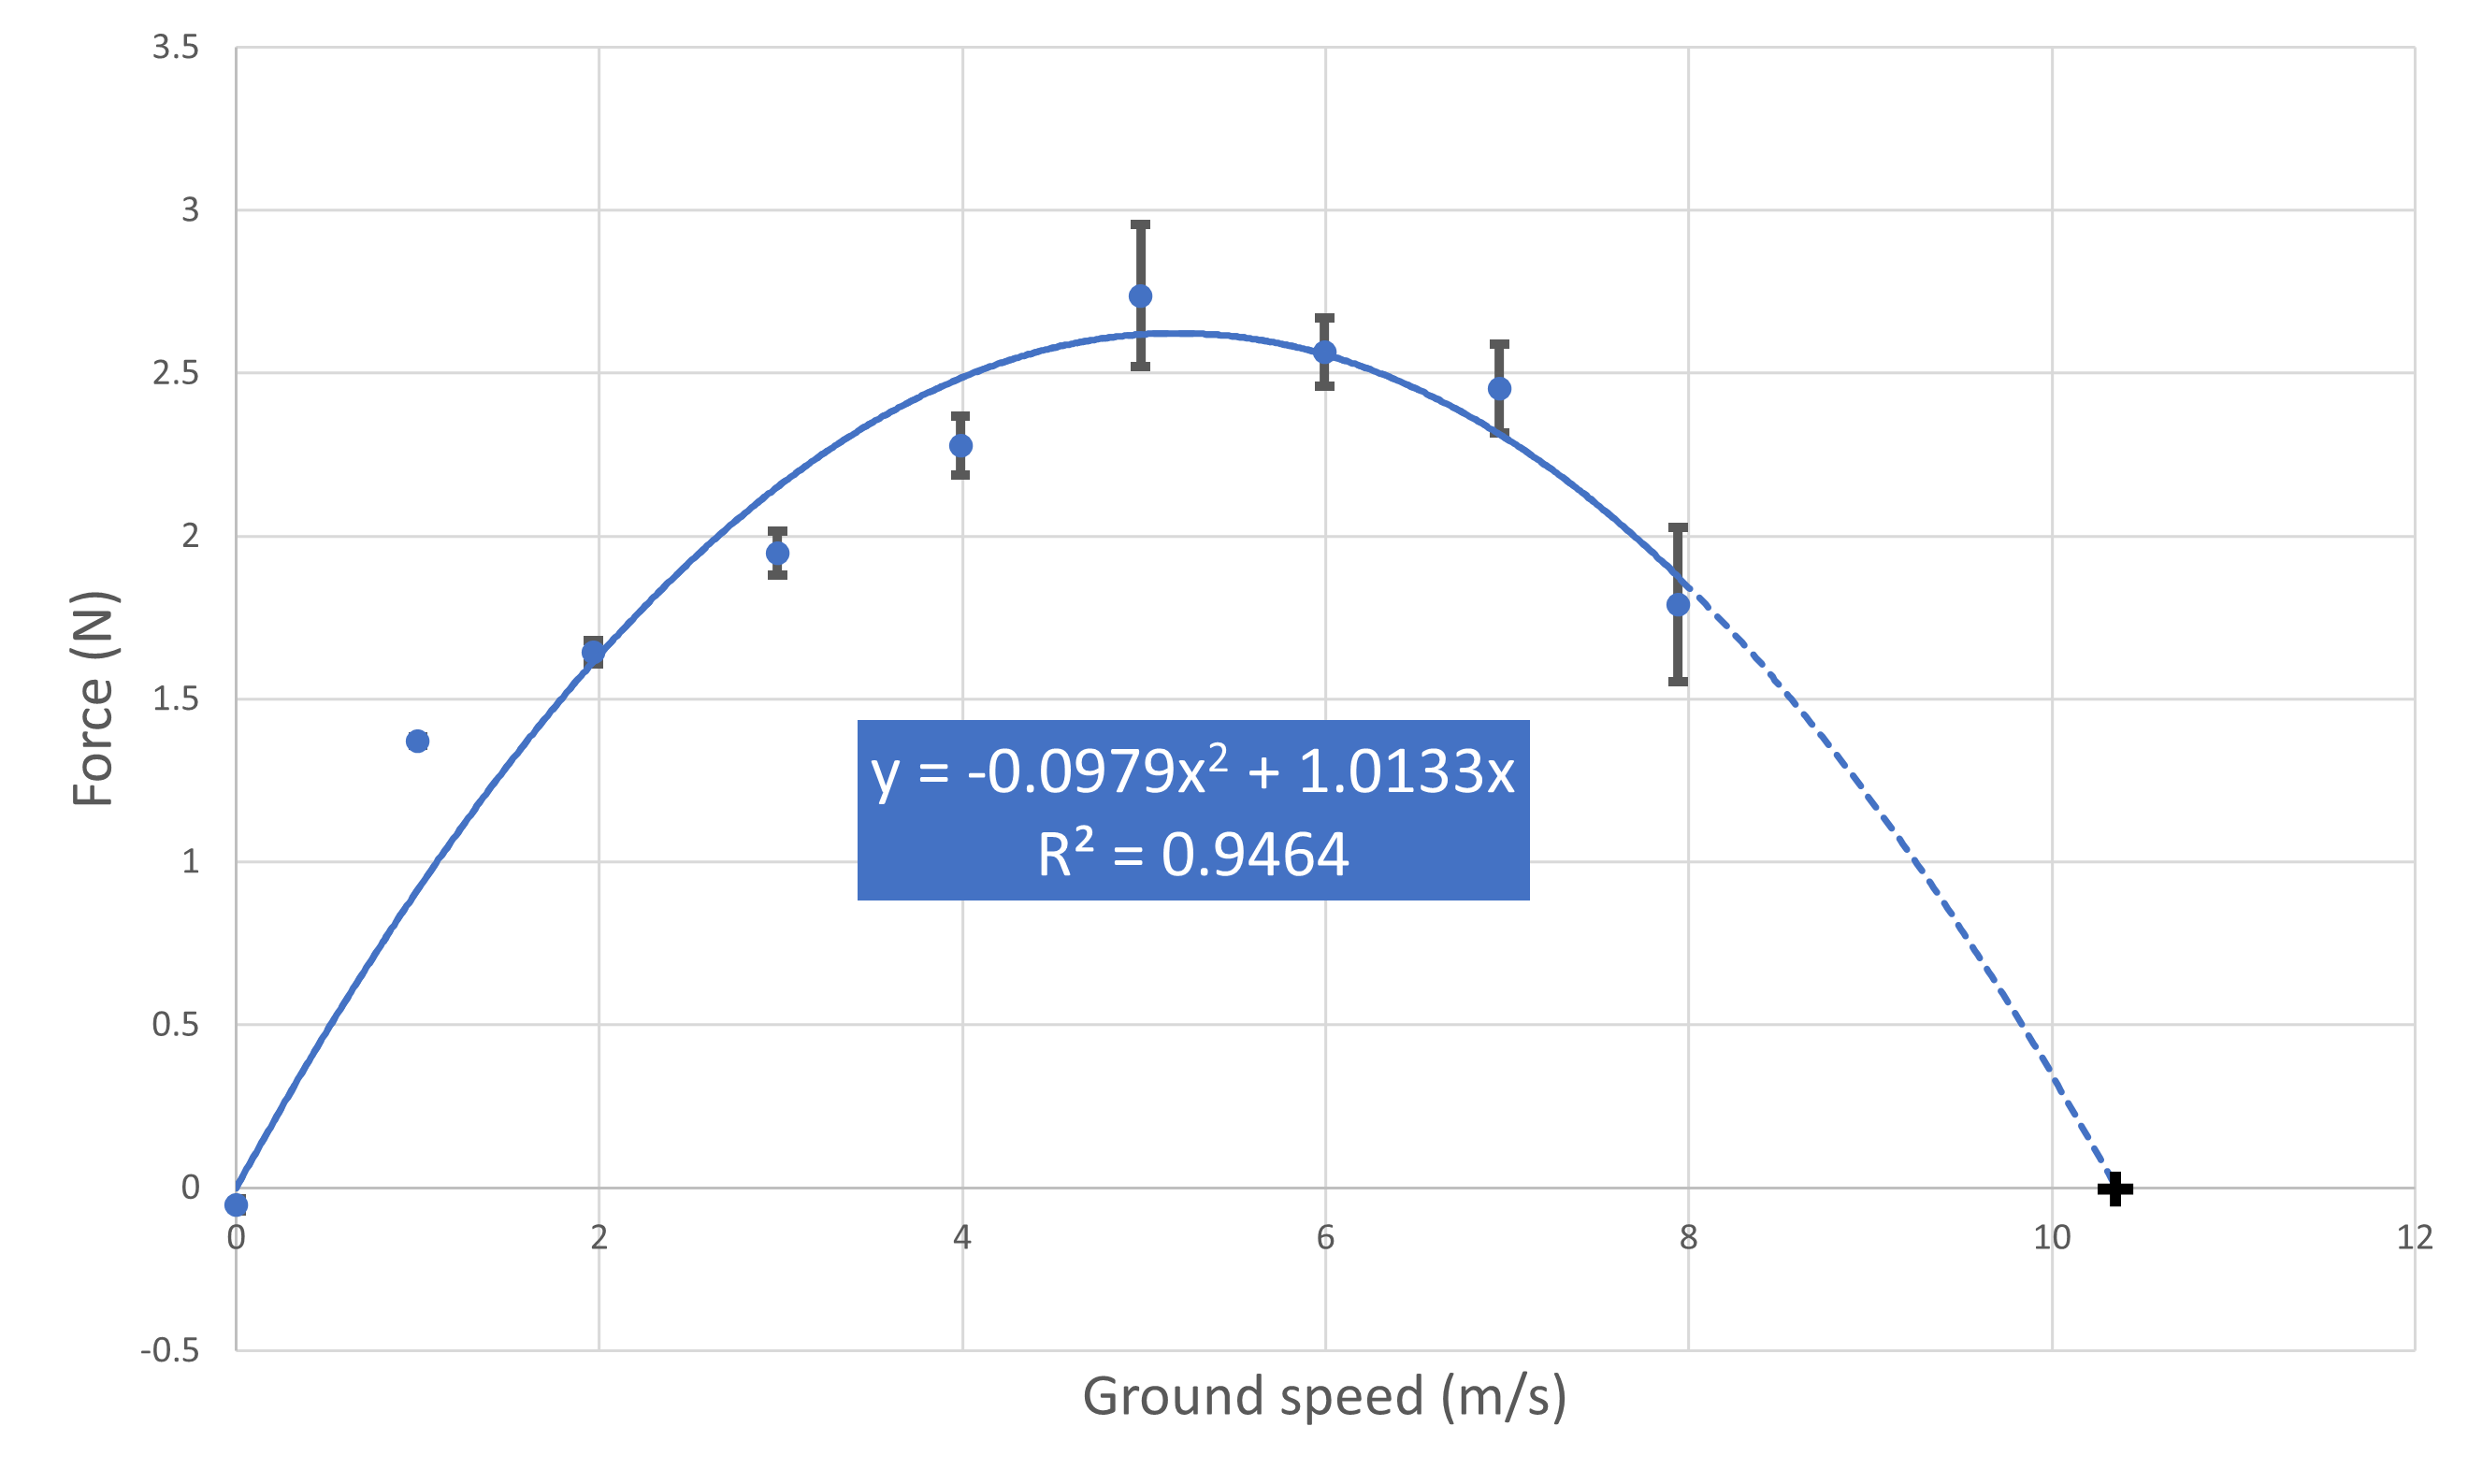
\includegraphics[width=0.9\linewidth]{images/part11/trendline.png}
    \caption{Configuration (D) - highest pitch force measurements with quadratic trendline}
    \label{fig:trendlineplot}
\end{figure}

Figure \ref{fig:synthesis}, displays a synthesis of the data acquired for the different blade pitch angles in the wind tunnel. First, due to structural flaws detailed earlier, the tests could not be conducted at maximum speed in all cases. Values up to 9 m/s could be obtained in the intermediate pitch case, and 8 m/s for the maximum pitch case. Although data points in those two cases were acquired over a smaller speed range, a predictable pattern could be observed. Overall, the data showed a thrust generation on the propeller’s part with a downwards trend of the total force at higher speeds and overall lower drag compared to configuration (C), without the propeller. 

\begin{figure}[!htbp]
    \centering
    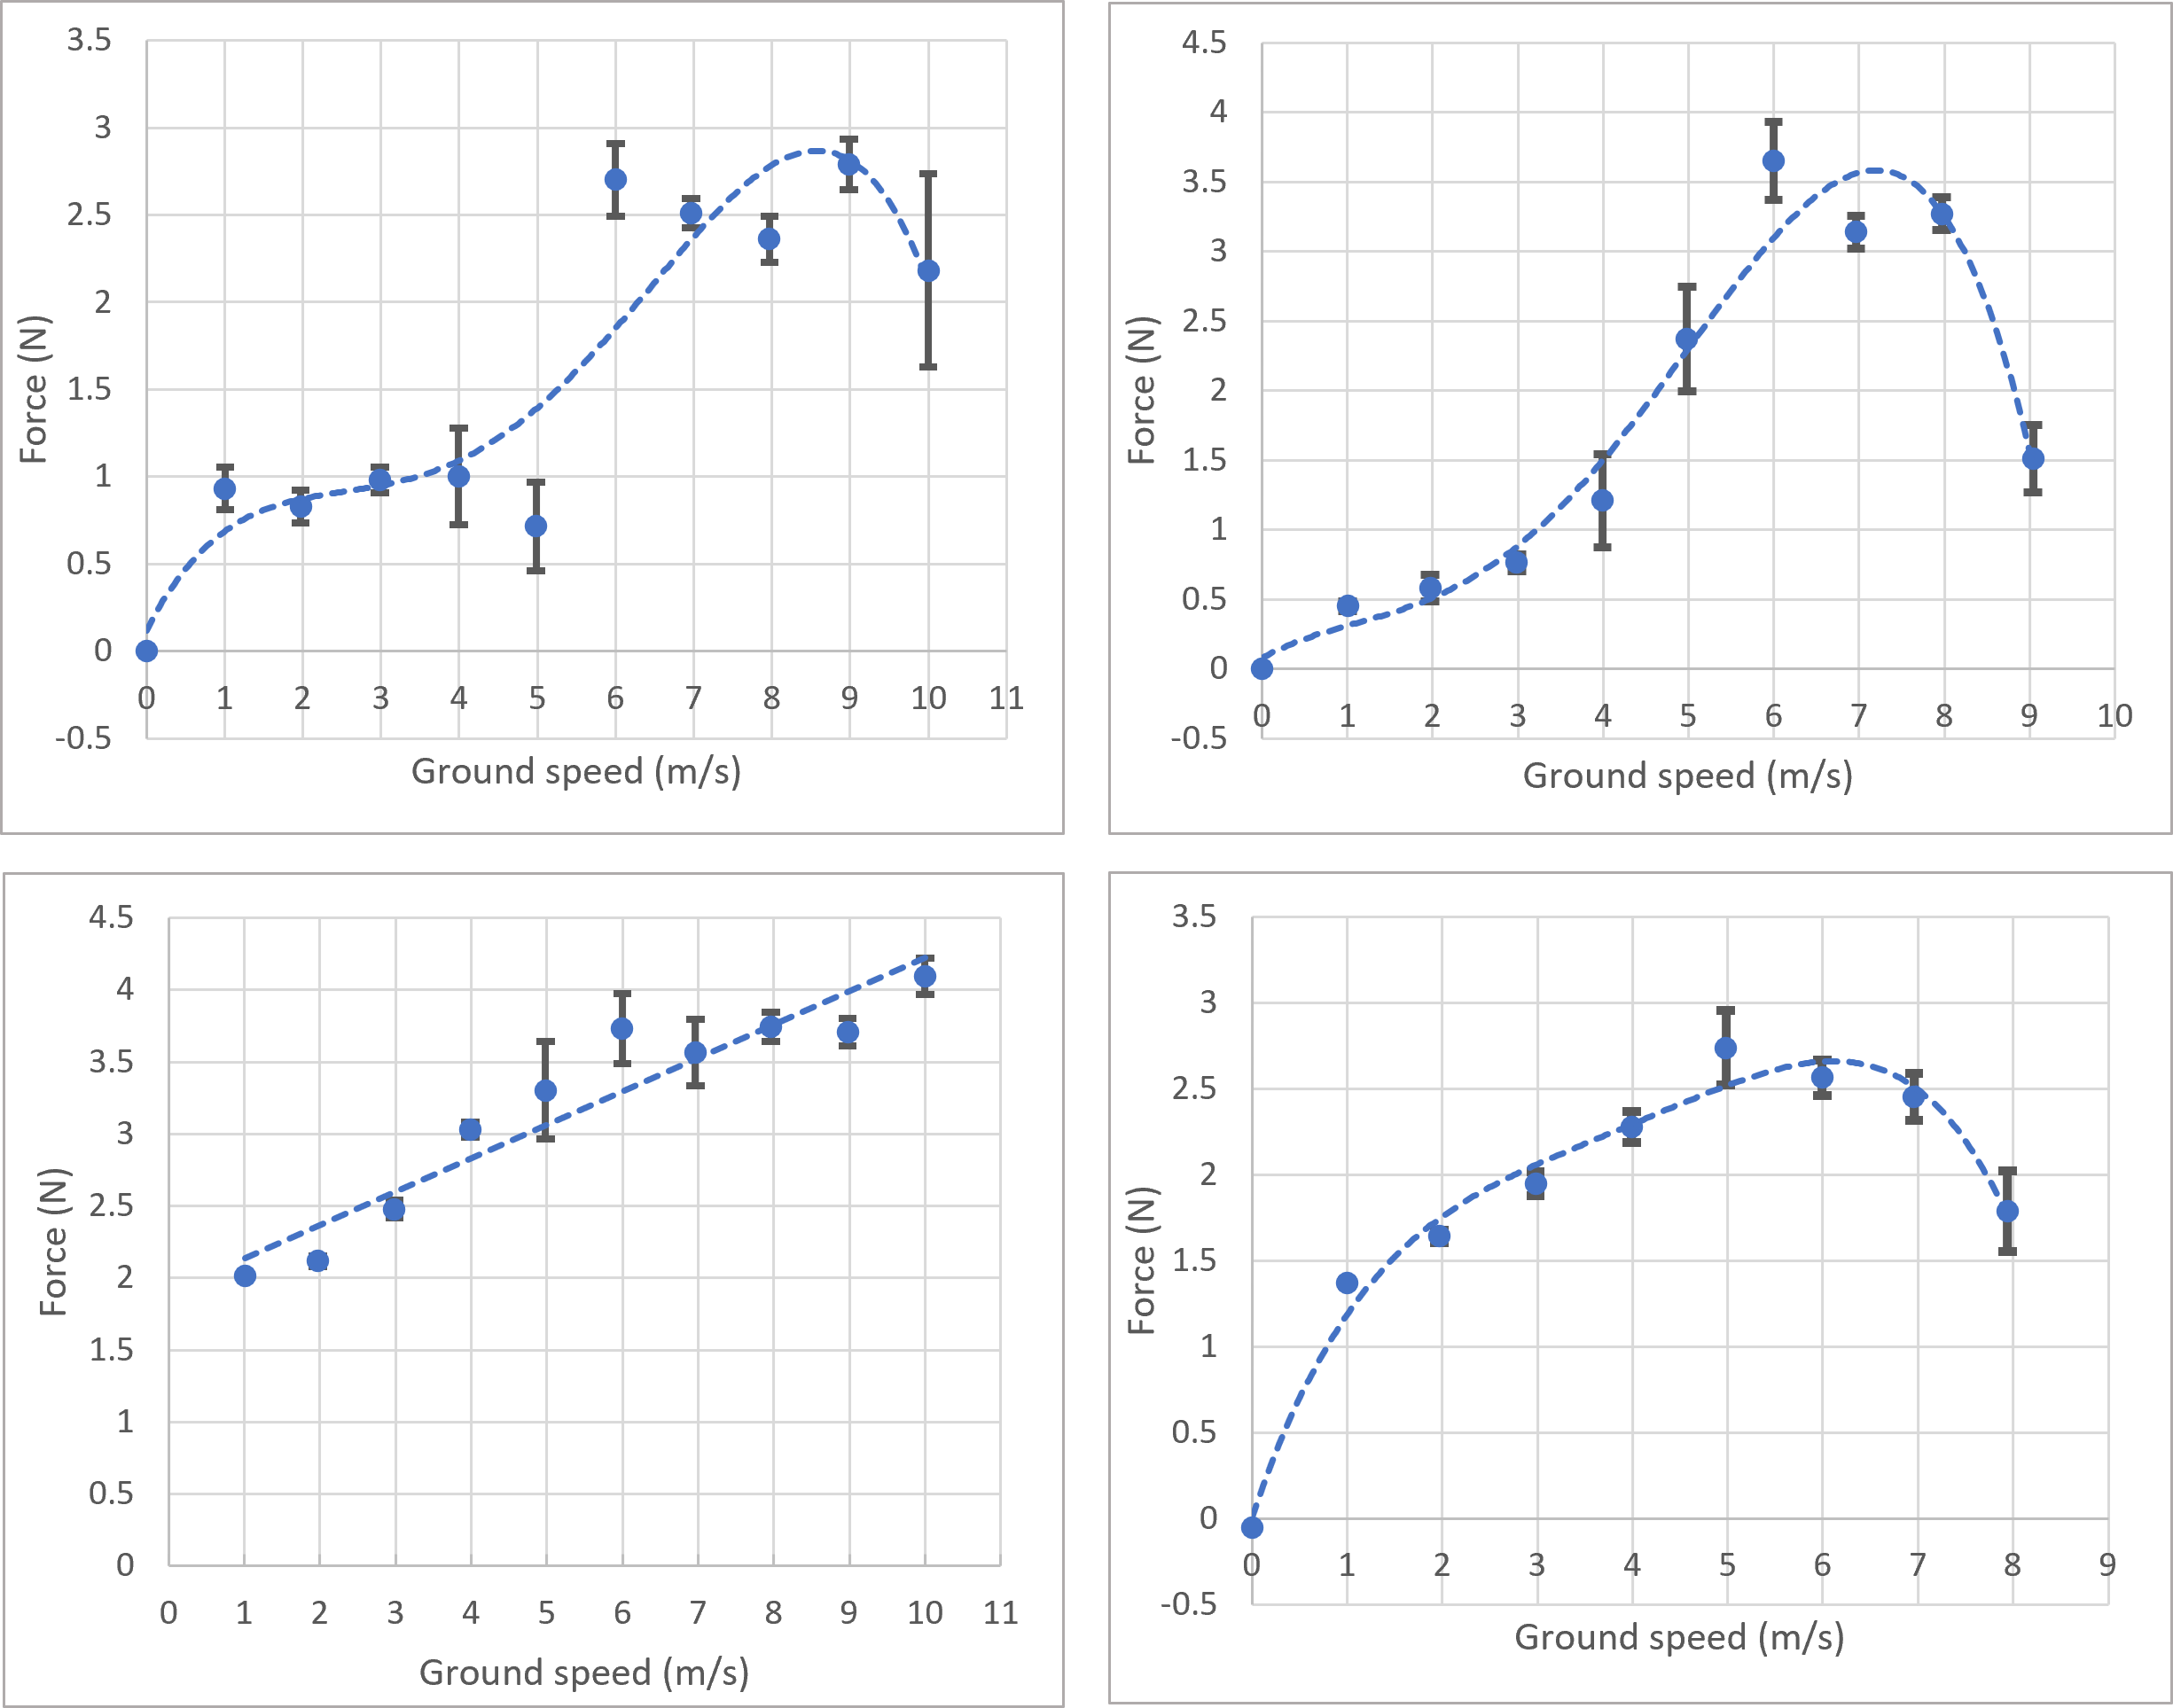
\includegraphics[width = \linewidth]{images/part11/individualresults.png}
    \caption{Time averaged total force on the vehicle as a function of the road speed. Configurations from top left to bottom right: (D) minimum pitch, (D) medium pitch, (C), (D) maximum pitch}
    \label{fig:individualresults}
\end{figure}

\begin{figure}[!htbp]
    \centering
    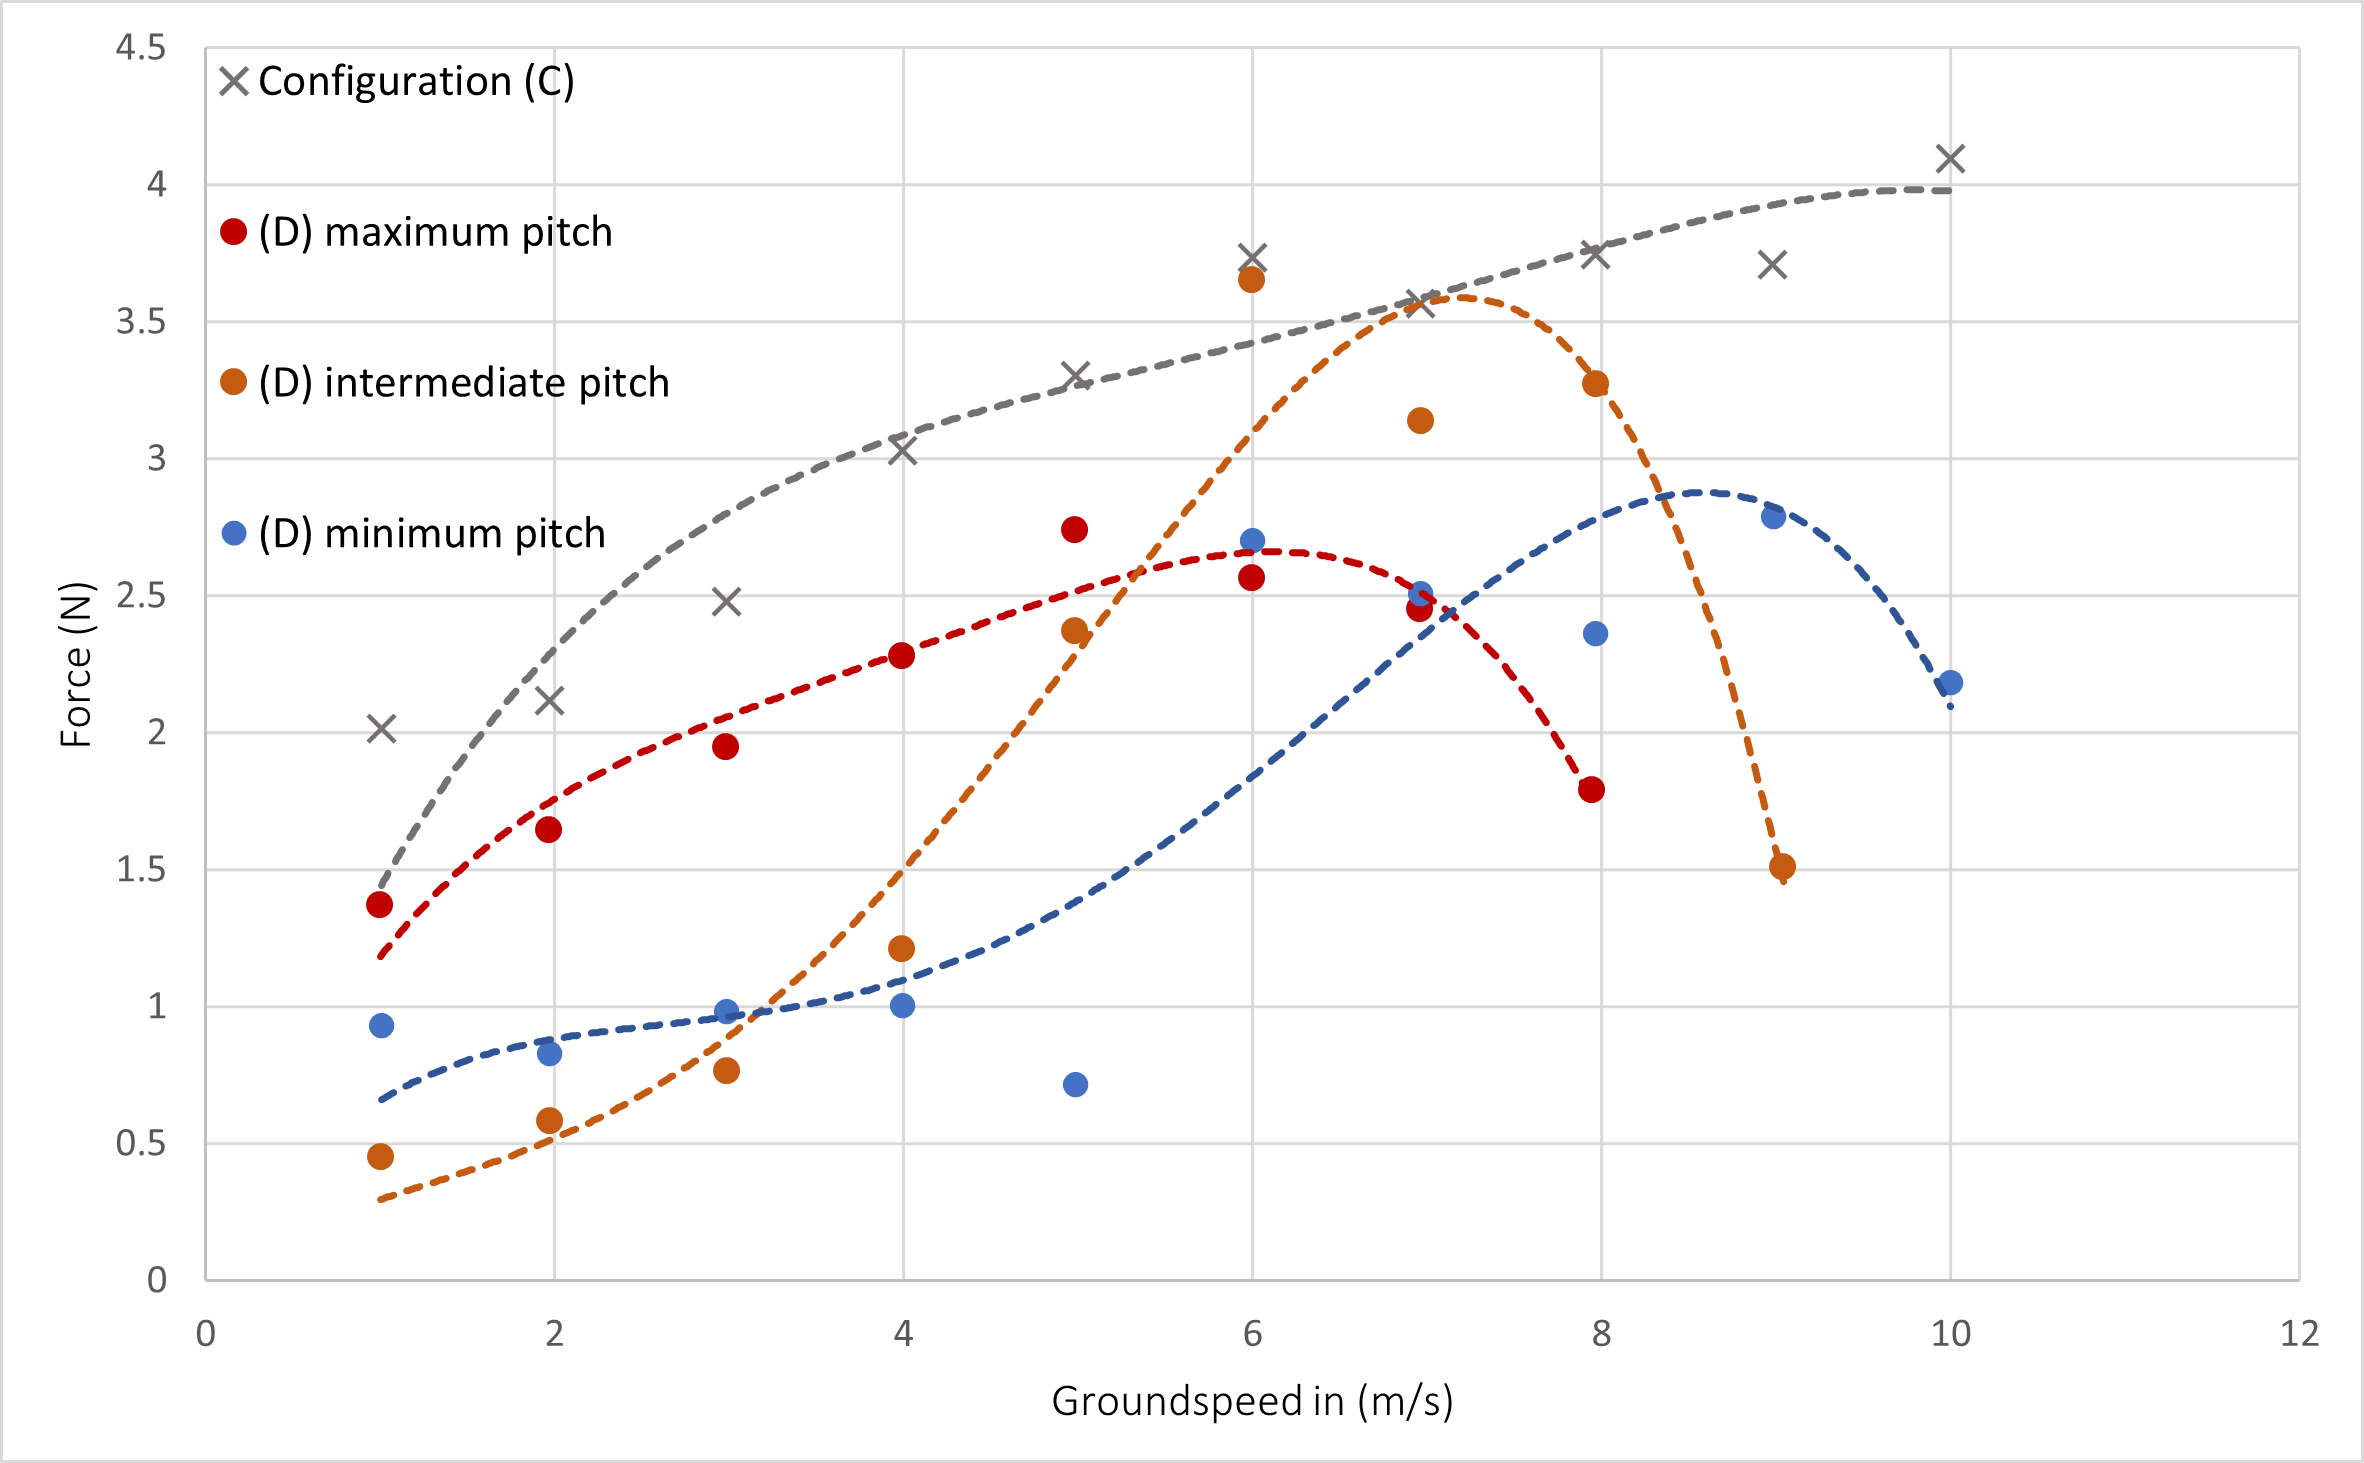
\includegraphics[width = 0.9\linewidth]{images/part11/synthesis.png}
    \caption{Total force as a function of speed for various configurations}
    \label{fig:synthesis}
\end{figure}


\begin{figure}[!htbp]
    \centering
    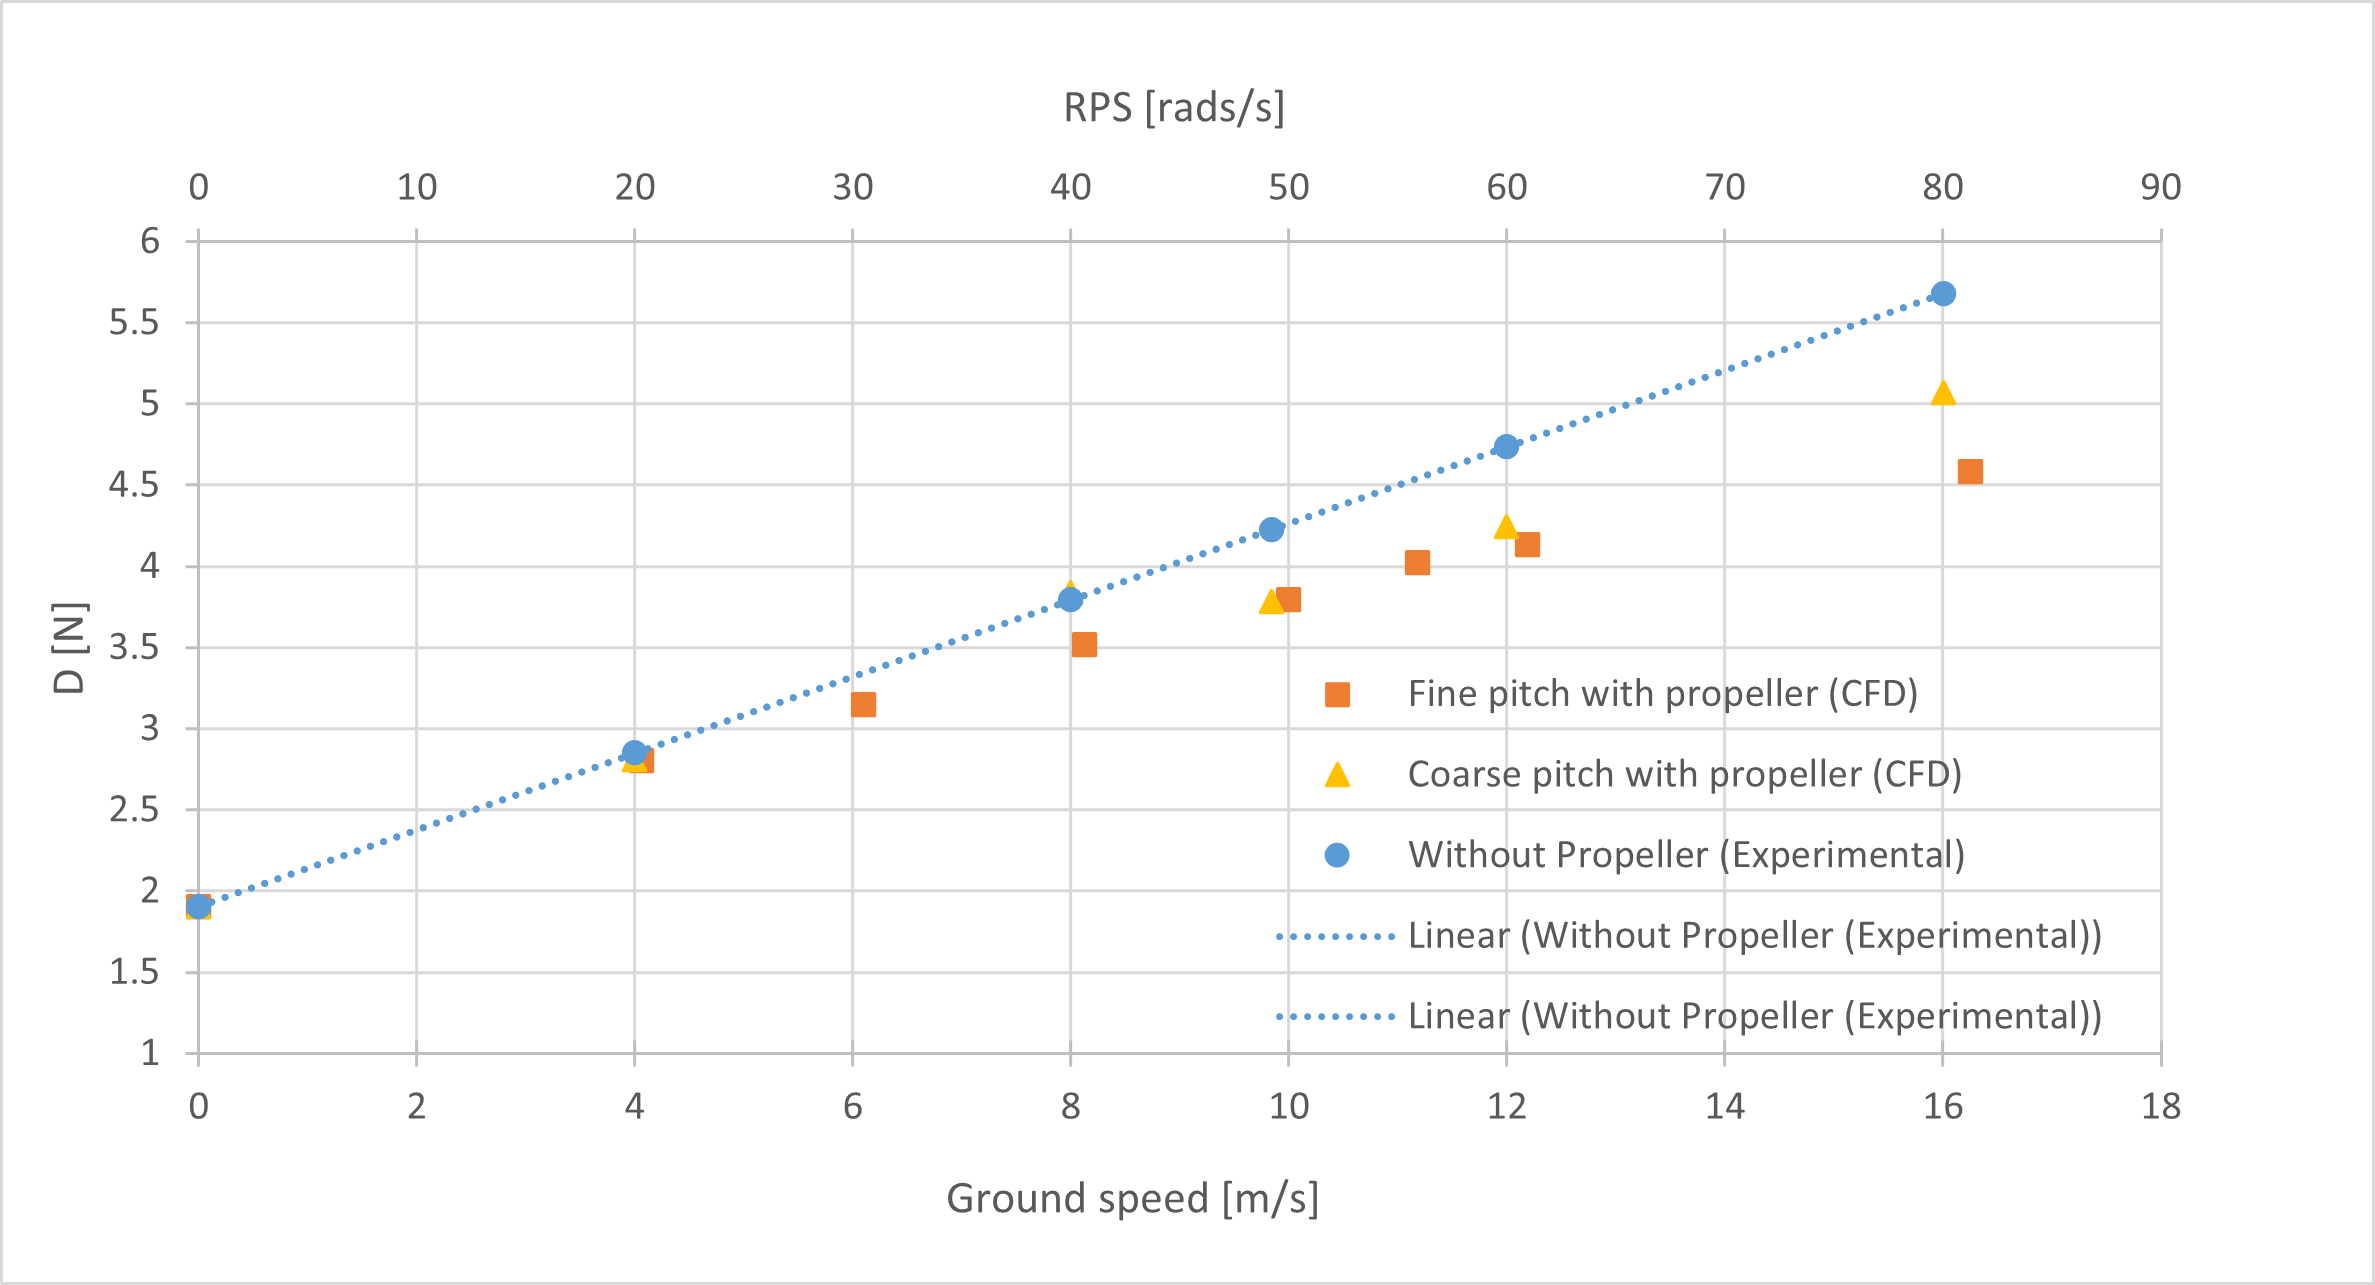
\includegraphics[width = 0.9\linewidth]{images/part10.1/Picture45.png}
    \caption{Plot of net drag D against rolling road speed (ground speed) with zero free stream velocity}
    \label{fig:d}
\end{figure}

\begin{figure}[!htbp]
    \centering
    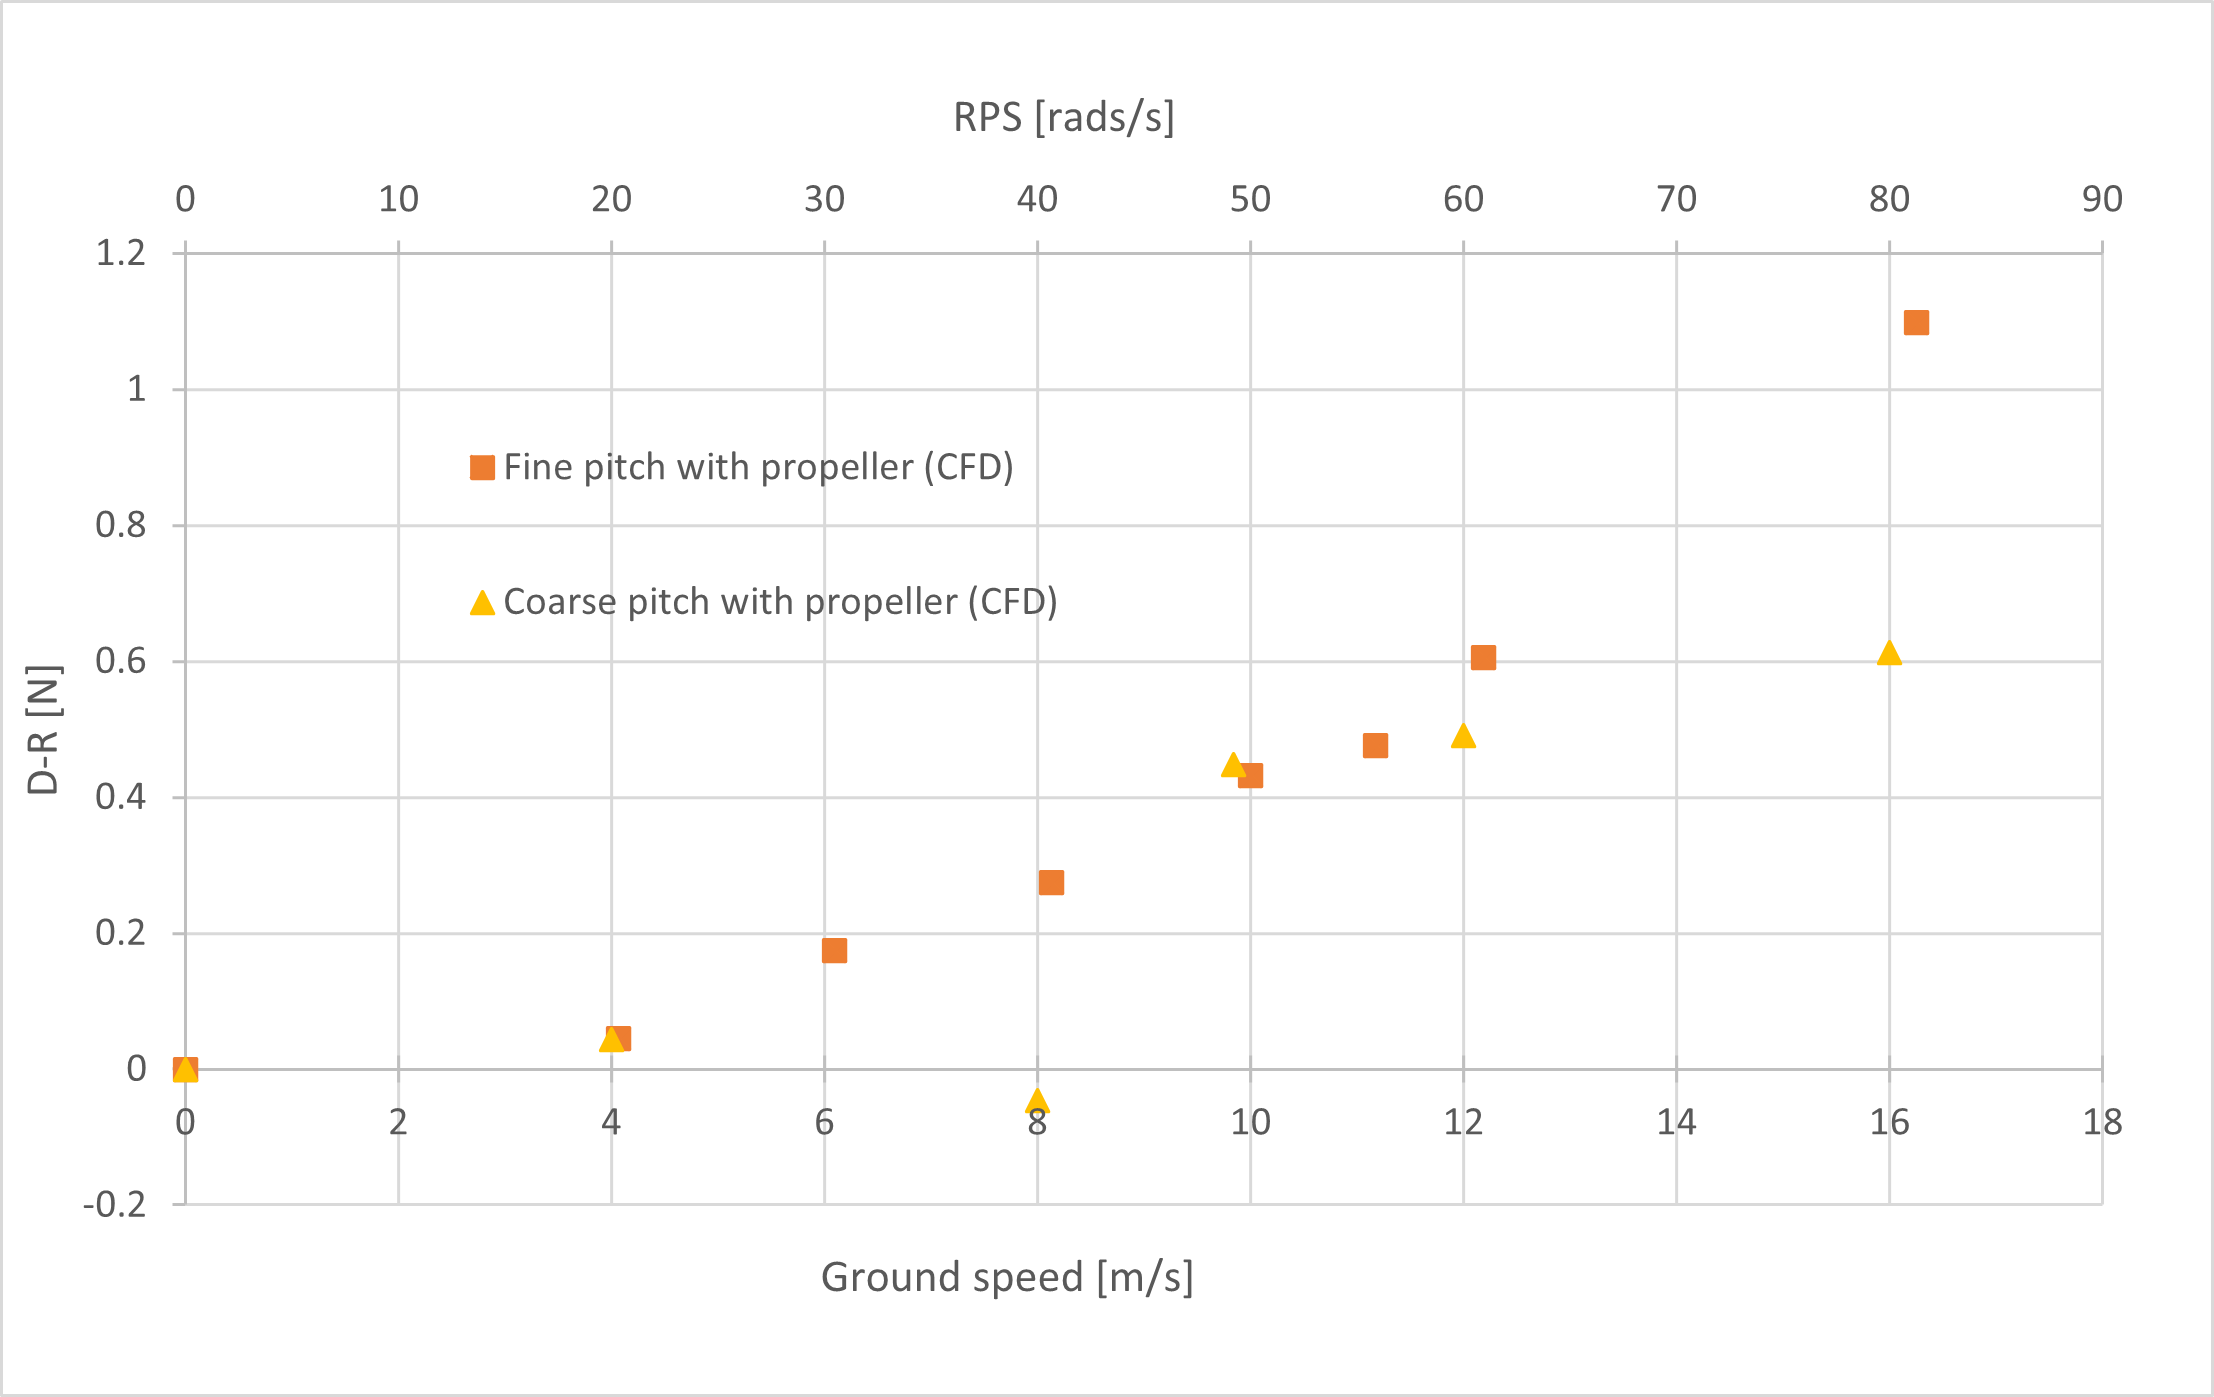
\includegraphics[width = 0.9\linewidth]{images/part10.1/Picture44.png}
    \caption{Plot of the negative of net drag –(D-R), the hypothetical vehicle thrust, against rolling road speed (ground speed)}
    \label{fig:dminusr}
\end{figure}

\begin{figure}[!htbp]
    \centering
    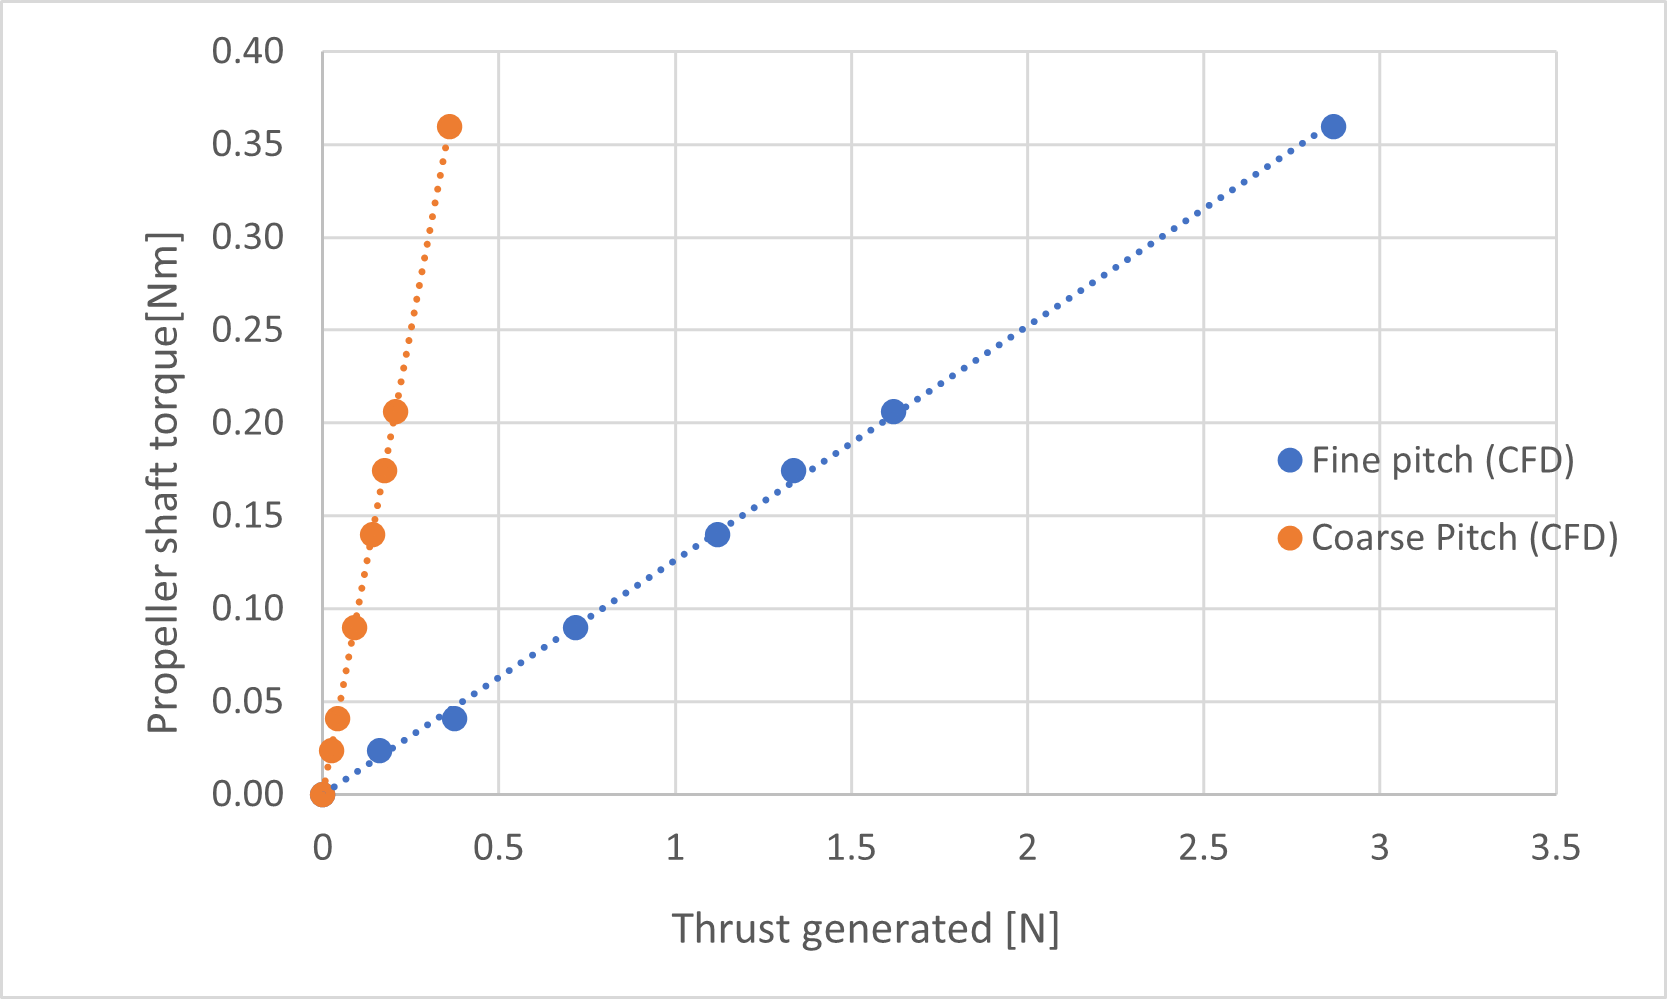
\includegraphics[width = 0.9\linewidth]{images/part10.1/prop_shaft_torque vs thrust.png}
    \caption{Plot of Propeller shaft torque against thrust generated. Note the steep gradient of the coarse pitch case}
    \label{fig:torquevsthrustprop}
\end{figure}

\begin{figure}[!htbp]
    \centering
    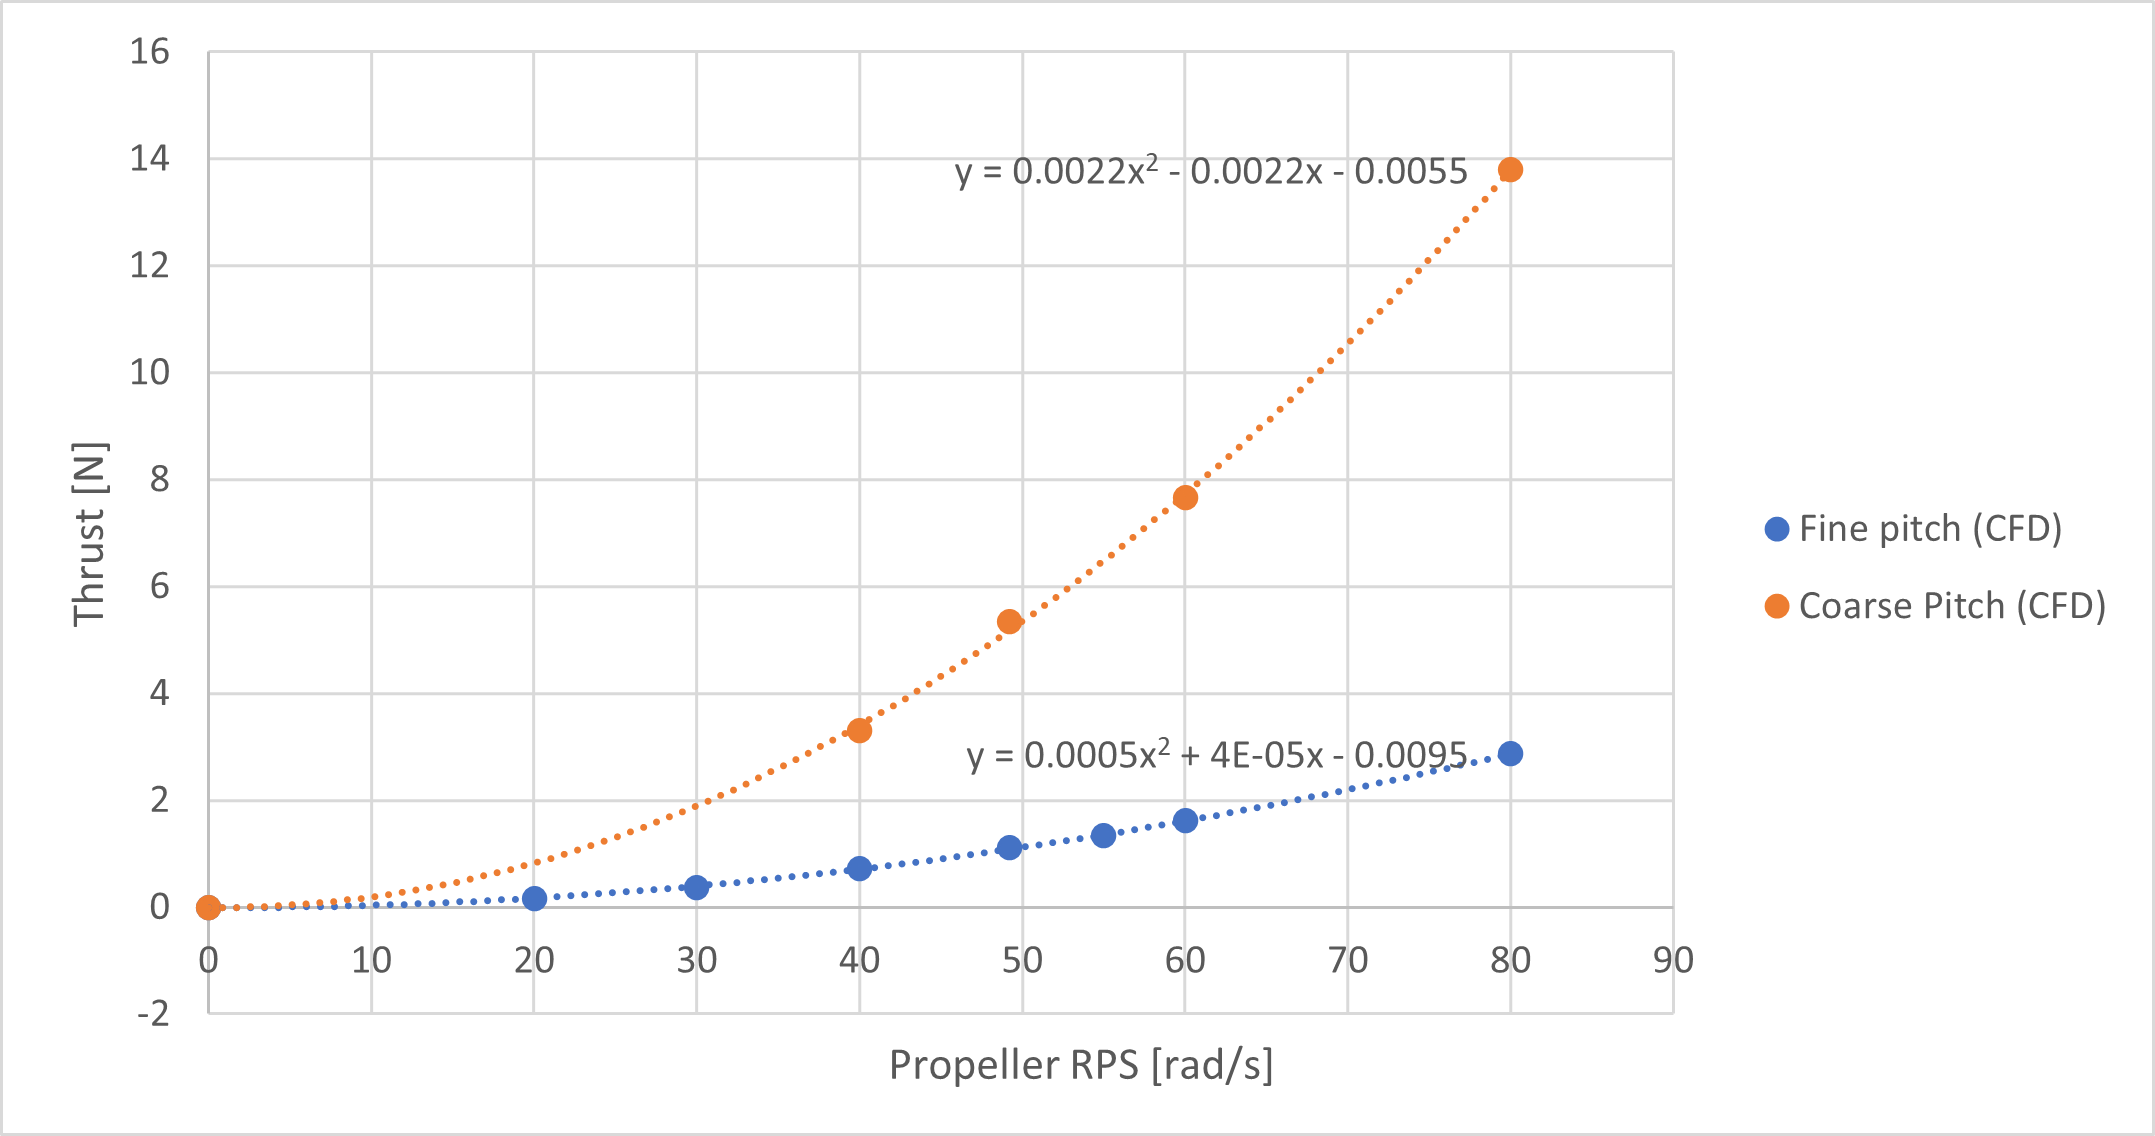
\includegraphics[width = 0.9\linewidth]{images/part10.1/thrustvsRPMplot.png}
    \caption{Plot of propeller thrust against propeller angular velocity in rad/s}
    \label{fig:thrustvsRPMplot}
\end{figure}

The results of the CFD analysis of propeller performance independent to the vehicle in Figure \ref{fig:thrustvsRPMplot} show a quadratic relationship with the propeller RPM. In Figure \ref{fig:torquevsthrustprop} The coarse pitch setup where the angle of attack of the propeller blade is high relative to the oncoming wind shows a much greater thrust curve at the cost of a large value of shaft torque. This can be analysed in more detail. The torque imposed on the shaft $\tau$ due to the rotation of the propeller independent of the vehicle can be represented as follows:

\begin{equation}
    \tau=r F
\end{equation}

Where $r$ is the radius of the wheels and $F$ is the resistance force this translates to at the contact point between the ground and tyre. 

\begin{equation}
    F=\frac{\tau}{r}
\end{equation}

The total drag of the vehicle can be written as $D=F+R$ where $R$ is the total resistance of the vehicle without the propeller mounted. 
The results for $R$ ,obtained in the RJ Mitchell wind tunnel, were used to find a line of best fit for the total rolling resistance, which was then used to calculate R. The values of calculated thrust from the CFD analysis, T can be added on to $D$ to show the effect of the propeller. The total drag is then calculated as follows:

\begin{equation}
    D = \frac{\tau}{r}+R
\end{equation}

In Figure \ref{fig:d}, the results of the combined drag $D$ have been plotted against rotation rate and equivalent rolling road ground speed. The values of $D$ under the blue line showing the best fit for the baseline resistance force without the propeller show a decrease in overall measured drag for both coarse and fine pitch cases. However, the coarse pitch case shows a higher drag $D$, indicating worse performance, despite the significantly larger values of thrust. The fine pitch case on the other hand shows a lower quantity in overall measured drag $D$ which can be seen clearly in ground speeds of 12 and above. This behavior can be explained by the plot of thrust against propeller RPM in Figure \ref{fig:torquevsthrustprop} . It can be observed from this plot that for the same value of thrust generated by the propeller, a larger torque is induced on the propeller shaft for the coarse case where the angle of attack is high on the blades. This is an indication that the propeller is not running efficiently.

The above results show that a decrease in total rolling resistance by optimization of the drivetrain, chain, bearings, and other components of the drivetrain can indeed allow a positive net thrust on the vehicle.  It is also in agreement with the experimental results both in terms of the result that lower overall drag is present with the propeller mounted compared to the baseline case, where the propeller is dismounted, and that the deviation from the baseline case increases at higher speed. By comparing experimental to CFD results it can be observed that the experimental data shows a more sudden deviation from the baseline after reaching approximately 6m/s whereas the transition is more smooth for the CFD case, which could be explained by a small amplitude resonance of forced vibration in the vehicle after the propeller was mounted. Overall it can be said though that both cases show that high angular velocity of the propeller is required in order to reach sufficient thrust. This behavior can be explained by the result that thrust increases with the square of the ground speed, shown in Figure \ref{fig:thrustvsRPMplot}, and that the higher the velocity, the greater the difference in rolling resistance to the thrust generated. The rolling resistance on the other hand increases linearly with ground speed, and therefore it can be concluded that a higher propeller RPM at the same ground speed would be an ideal situation where rolling resistance practically is kept constant. 

Equation 20 also shows that a larger wheel radius $r$ means the wheels transmit this torque as a smaller force to the ground. It is therefore reasonable to state that for the case of zero relative wind speed where the aerodynamic drag acting on the wheels is less significant, larger wheels should help decrease the adverse effect of the propeller. 

In Figure \ref{fig:dminusr} the same values of total drag $D$ have been plotted against rolling road speed. This shows a hypothetical situation where the rolling resistance of the vehicle is zero, which is the theoretical limit of the drivetrain performance. This assumes the resistance in the bearings, tyres, chain, and drivetrain components are zero and that the propeller performance alone is considered. Using this hypothetical condition, it can be predicted that for the same conditions for the propeller arrangement, a net positive thrust can indeed be achieved. At the same time, it is clear that the propeller efficiency is pivotal in achieving this result. The higher this efficiency is, the greater the amount of rolling resistance that can be offset and therefore produce a net positive thrust. Also, the deviation of the thrust from zero thrust is proportional to the square of the velocity, and therefore one can easily assume that the higher RPM, the higher the blade speed, and therefore larger net thrust.


\begin{figure}
    \centering
    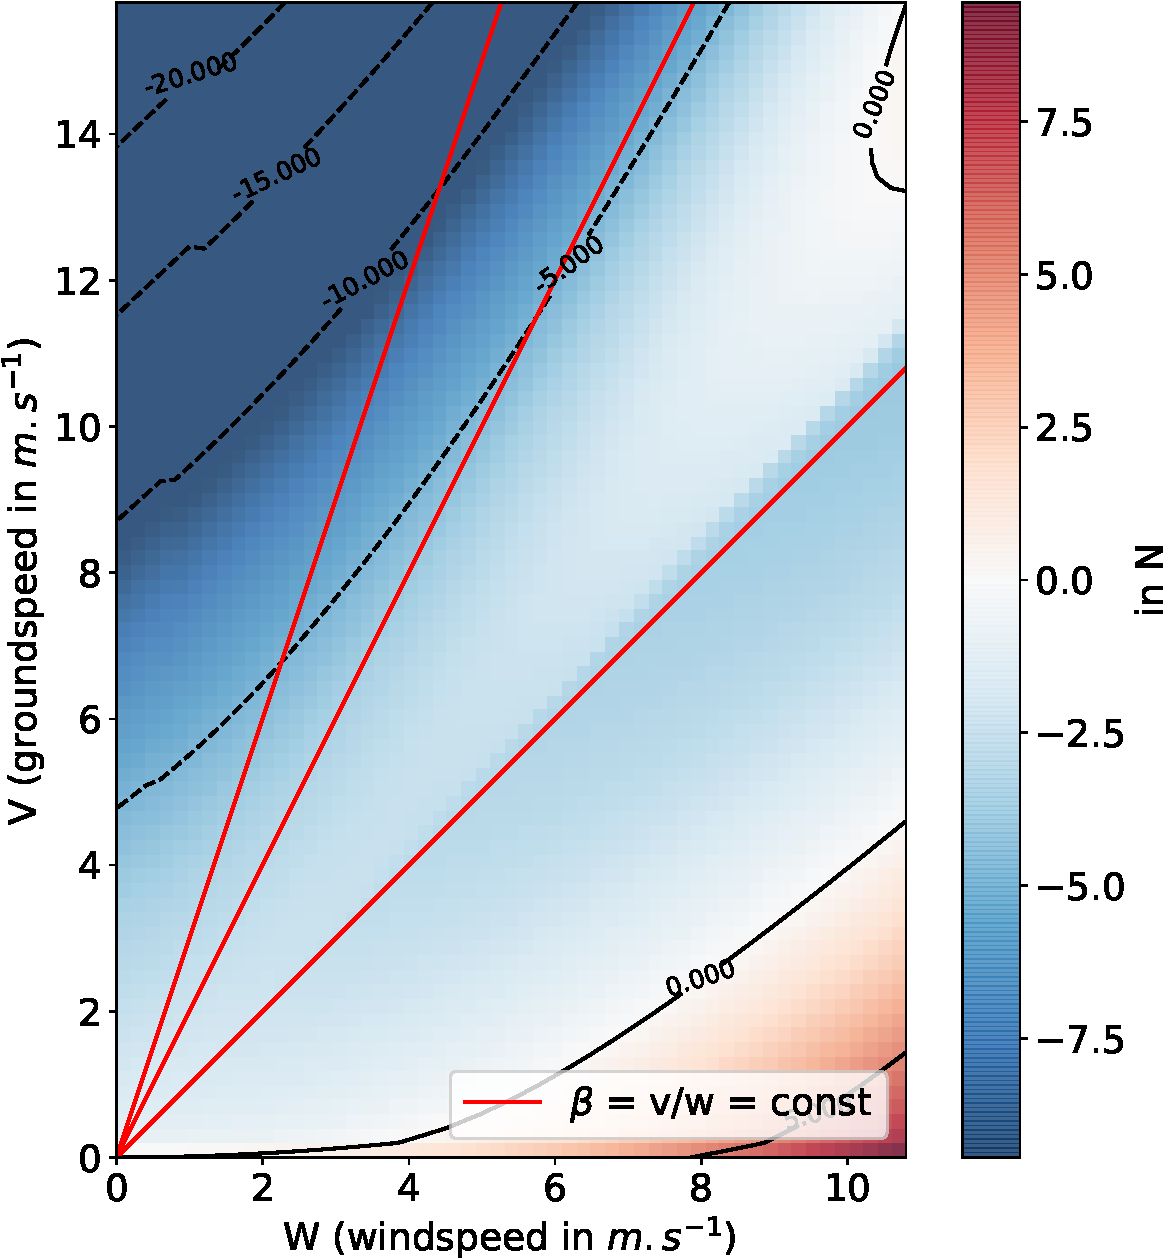
\includegraphics[width = 0.447\linewidth]{images/part11/expe.pdf}
    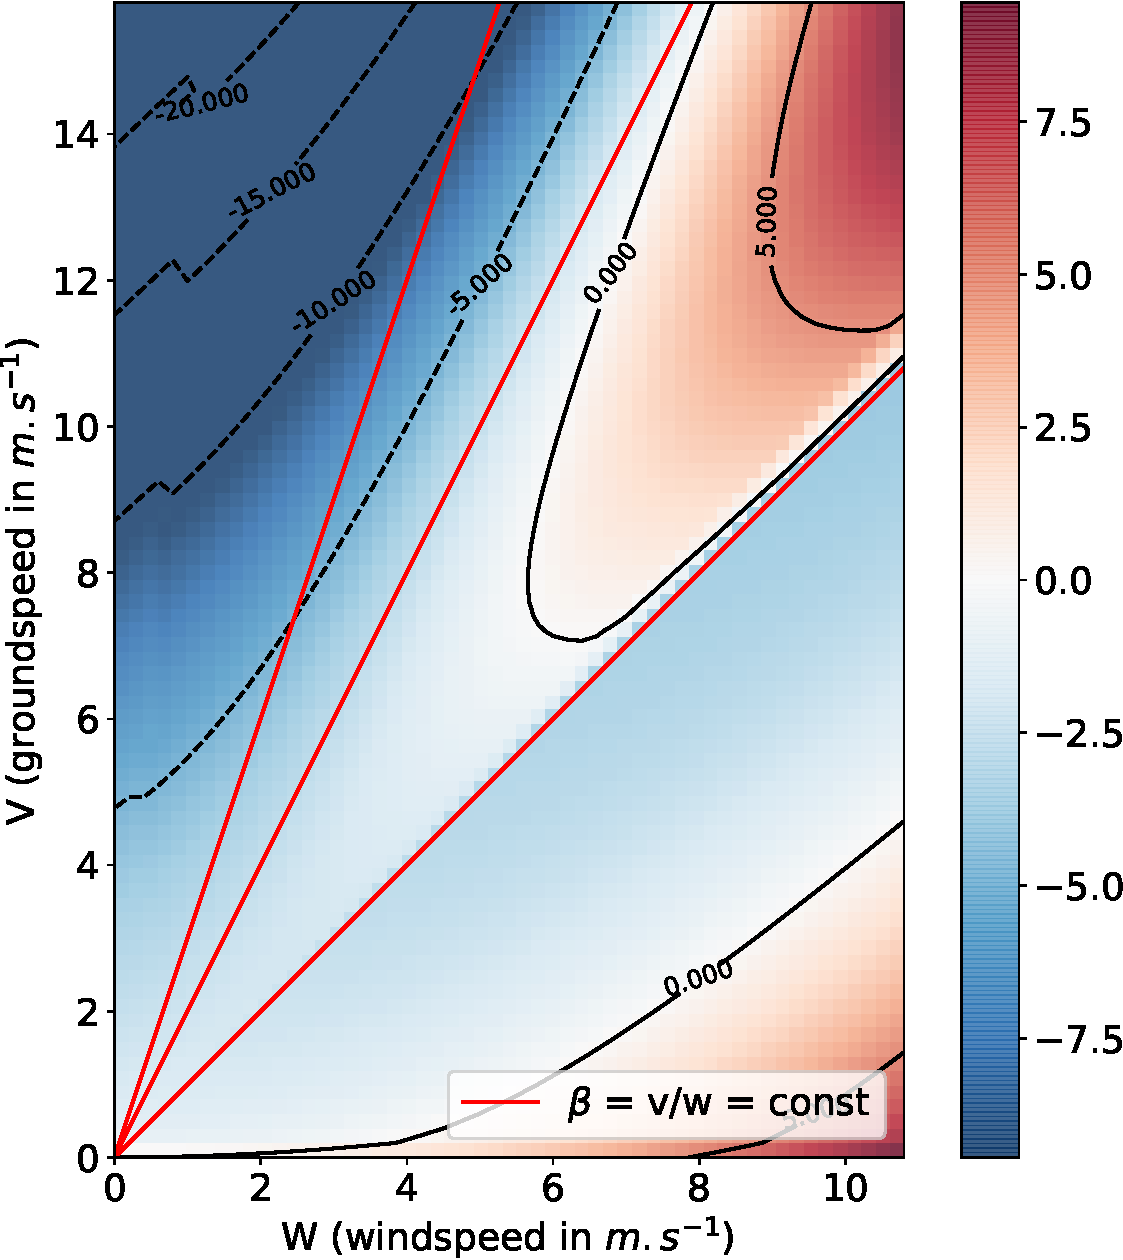
\includegraphics[width = 0.43\linewidth]{images/part11/expebigger.pdf}
    \caption{Total force contours using experimentally acquired rolling resistance and drag curves. Manufactured propeller (left) and larger diameter propeller (1.2m) (right)}
    \label{fig:expecontours}
\end{figure}

Figure \ref{fig:expecontours}.1 shows the force contour obtained when plugging in the experimental values for drag and rolling resistance. The difference from what was acquired in Figure \ref{fig:pythonresults} mainly comes from the rolling resistance. The rolling resistance of the vehicle was much higher than anticipated. This graph shows that even if the propeller had performed as expected, the wind speed would not have been reached. 

It is also observed in this figure that the closest point to the origin where the force becomes positive is off the $V/W=1$ axis. This is due to the pitch of the propeller. It stems from the propeller’s thrust to torque ratio being slightly better for higher inflow (allowed by a higher $V/W$ ratio). Increasing the pitch angle would increase the value of the polar coordinate of this point. Likewise in the other direction.

As shown comparing the contours in Figure \ref{fig:expecontours}, increasing the propeller size would lead to better performance of the vehicle. This is due to the propeller being able to generate more thrust for equal efficiency. Therefore, even in this case where the same thrust to torque ratio was maintained, the force delta $F_{net}$ was greater in magnitude and outweighed the drag and rolling resistance forces.

This concludes that a high RPM must be maintained while keeping the same propeller efficiency and low resistance. Therefore when optimising the vehicle to go faster than the wind, one must prioritise RPM, which practically means the use of a high gear ratio while maintaining adequate propeller and drivetrain performance. 

Furthermore, maximising the propeller diameter to vehicle weight and size ratio would allow the net force defined earlier $F_{net}$ to be more significant in comparison to the resisting forces, namely drag and rolling resistance. This would mean that higher performance could be achieved over the whole domain of operation.


\subsection{Vehicle drag assessment}

\begin{figure}[!htbp]
    \centering
    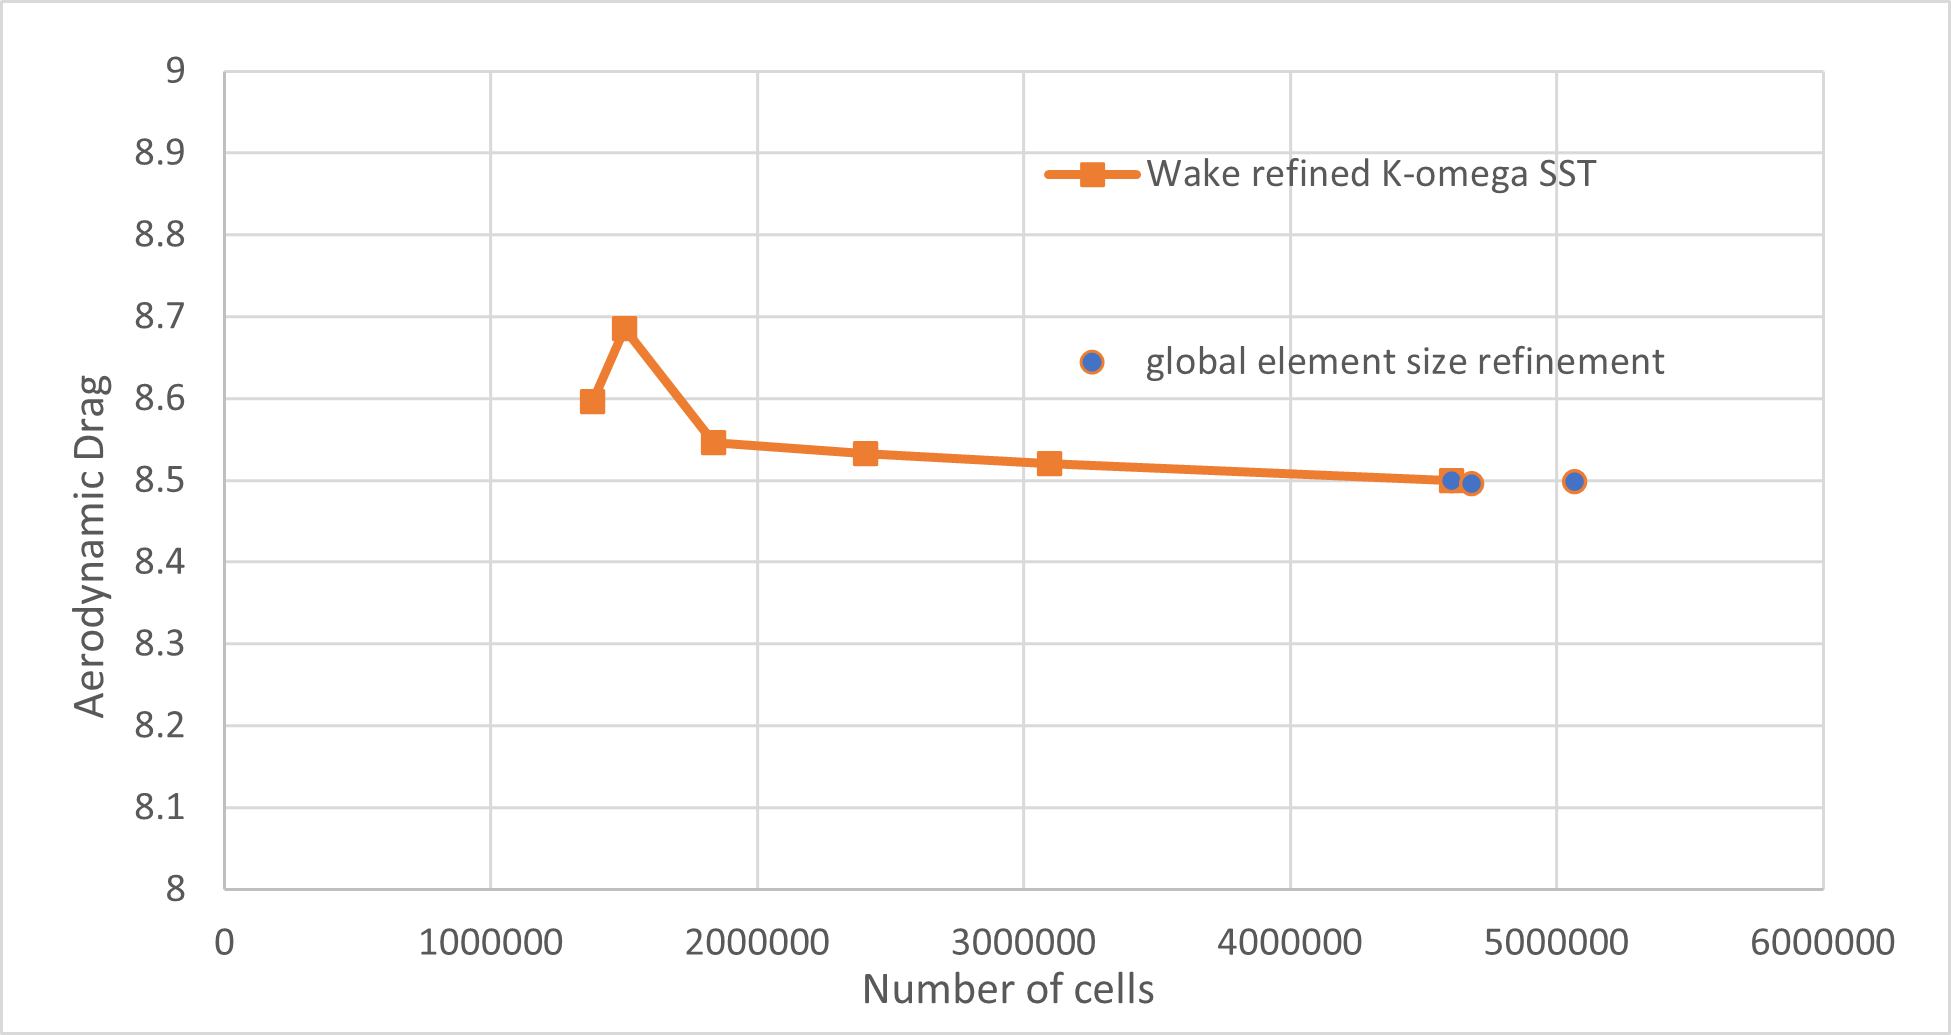
\includegraphics[width=0.8\linewidth]{images/part10.1/dragncells.png}
    \caption{Sensitivity of Drag at $10m/s$ of the vehicle in response to wake refinement followed by global element size refinement}
    \label{fig:dragncells}
\end{figure}

\begin{figure}[!htbp]
    \centering
    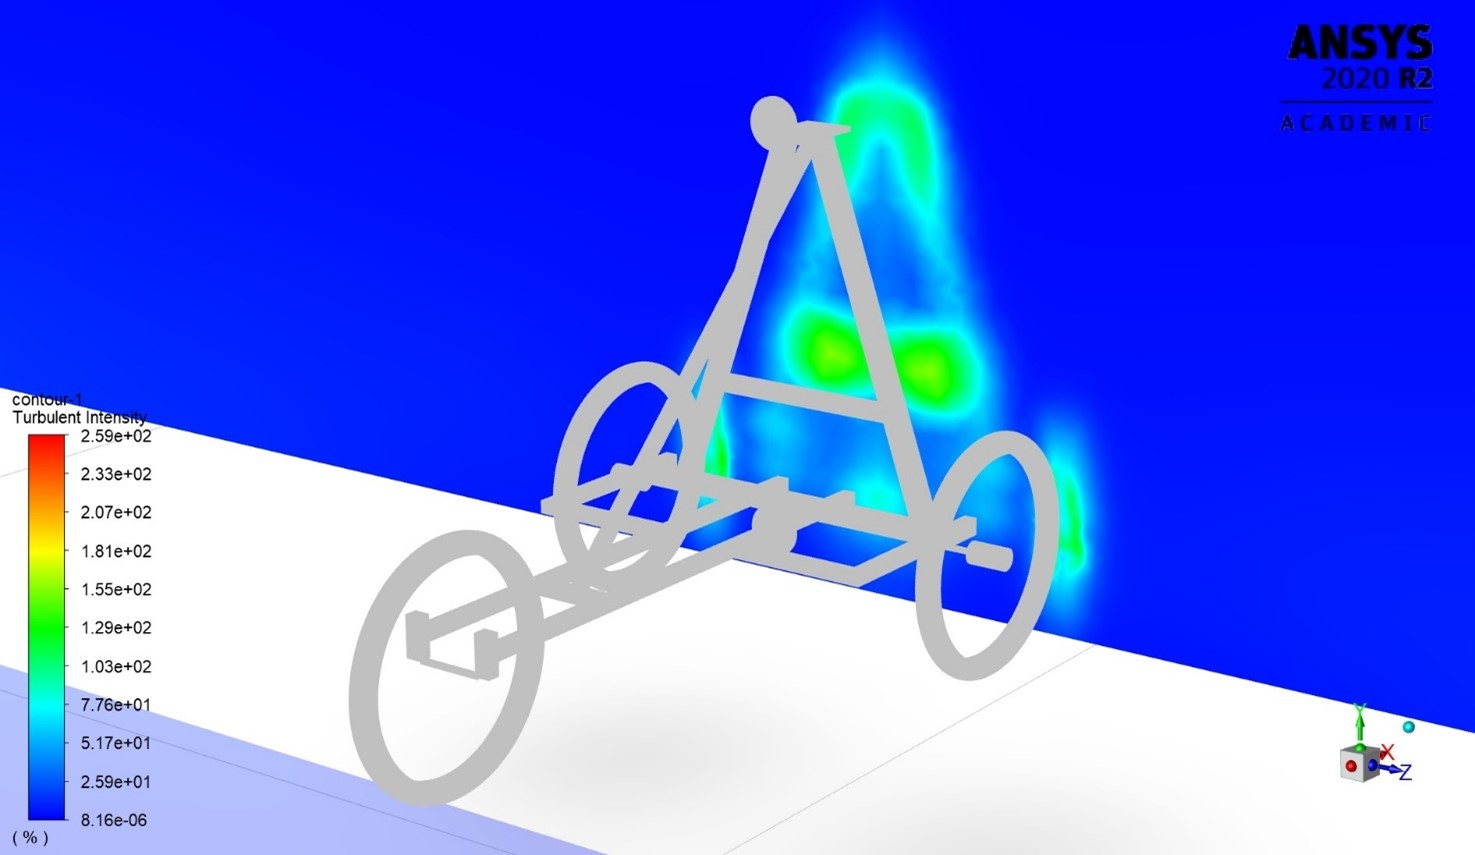
\includegraphics[width=0.8\linewidth]{images/part10.1/vehicleiso.jpg}
    \caption{Contour plot of turbulence intensity the wake on a surface normal to the direction of the free-stream velocity and coincident with the plane of the propeller}
    \label{fig:vehicleiso}
\end{figure}

Figure \ref{fig:dragwind} shows a plot of drag force of the vehicle at various speeds from a range of 0 to 10 m/s. The results in general show a small over-prediction in drag but are in close agreement with the experimental results. 

\begin{figure}[!htbp]
    \centering
    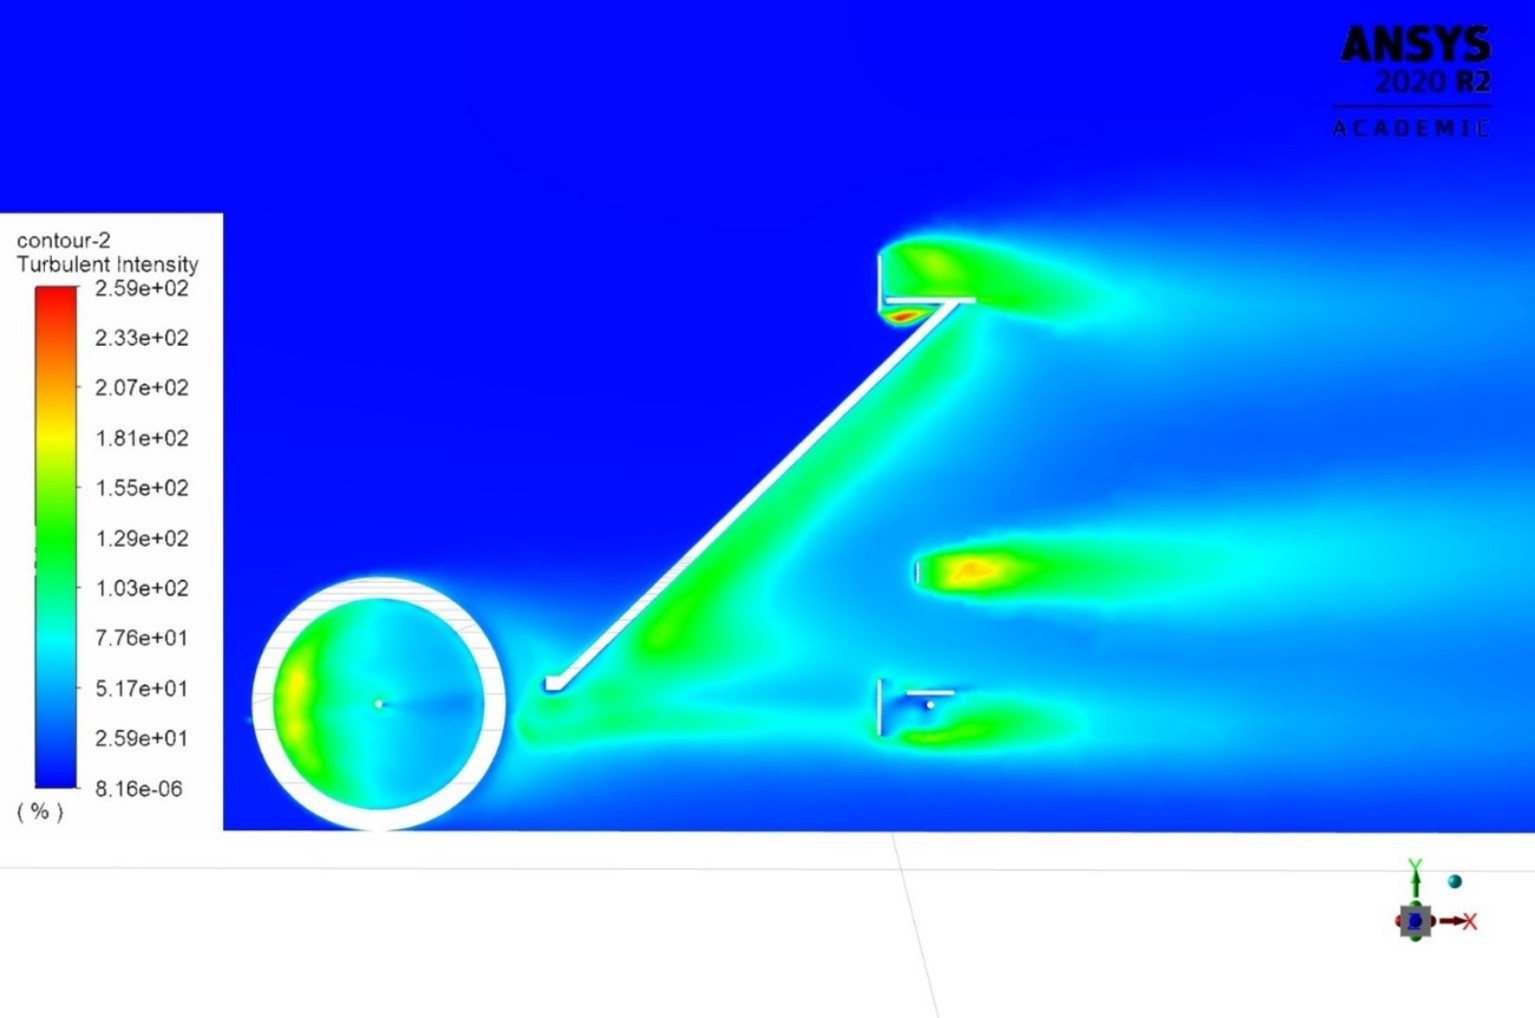
\includegraphics[width=0.8\linewidth]{images/part10.1/vehicleside.jpg}
    \caption{Contour plot of turbulence intensity the wake on a surface normal to the direction of the free-stream velocity and coincident with the plane of the propeller}
    \label{fig:vehicleside}
\end{figure}

\begin{figure}[!htbp]
    \centering
    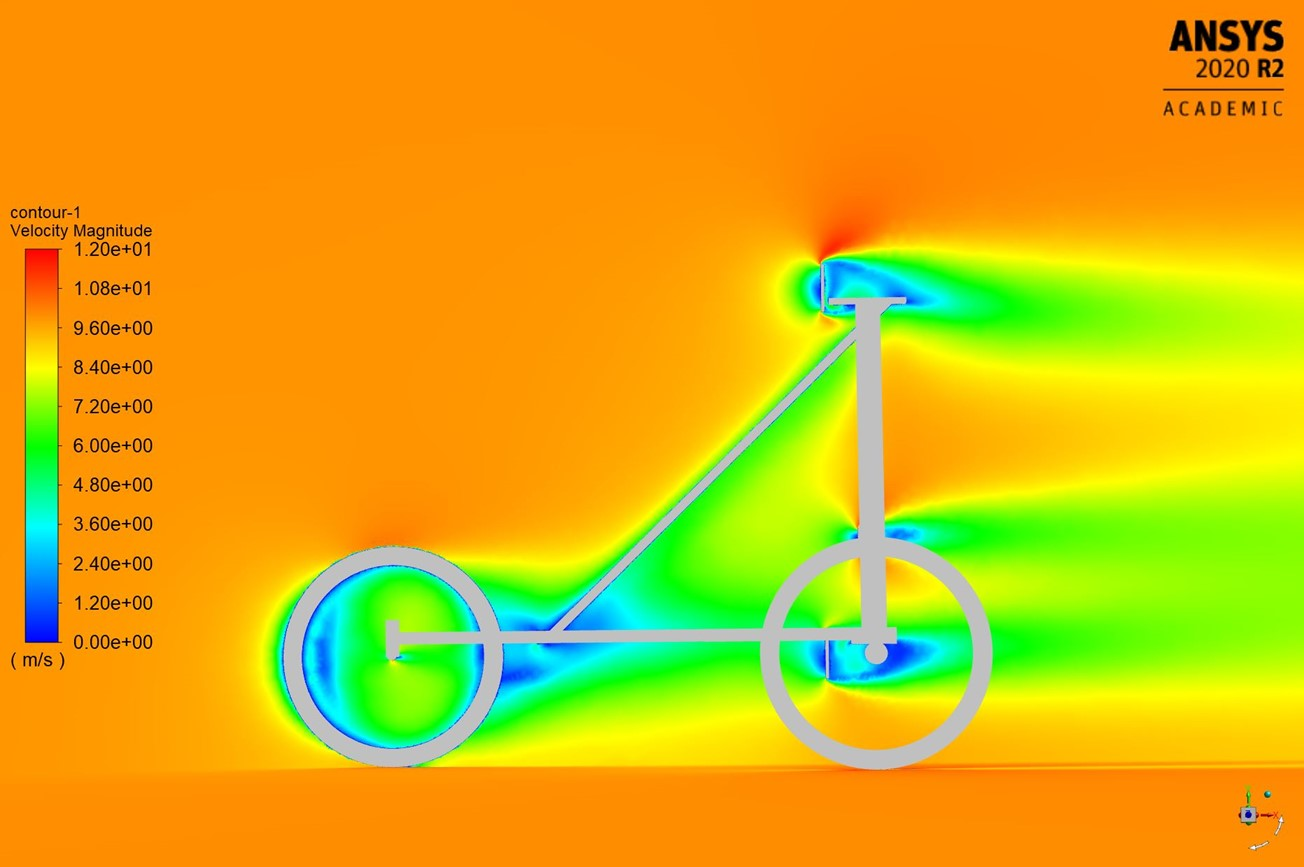
\includegraphics[width=0.8\linewidth]{images/part10.1/vehiclesidevelocity.jpg}
    \caption{Contour plot of the velocity magnitude on the symmetry plane of the vehicle}
    \label{fig:vehiclesidevelo}
\end{figure}

\begin{figure}[!htbp]
    \centering
    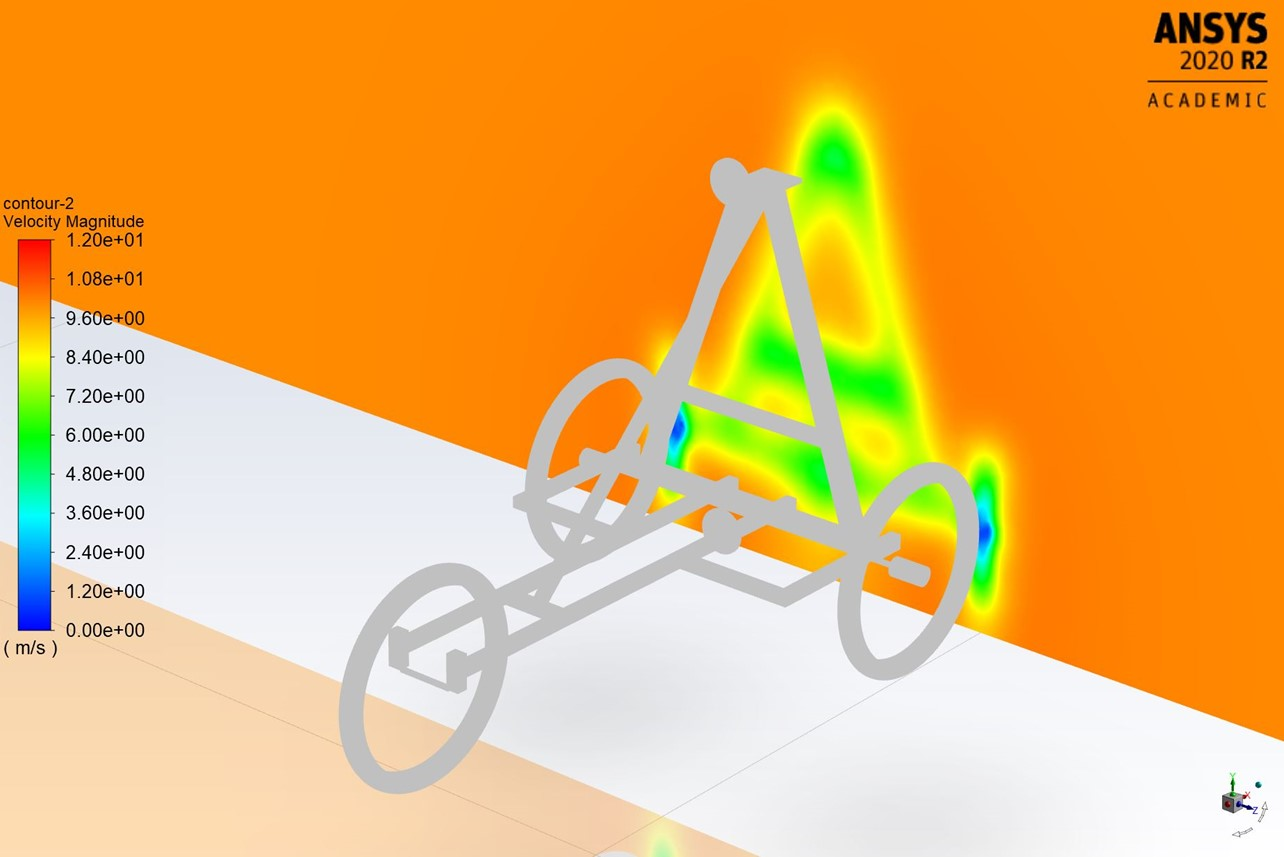
\includegraphics[width=0.8\linewidth]{images/part10.1/vehicleisovelocity.jpg}
    \caption{Contour plot of velocity magnitude in the wake on a plane coincident to the plane of the propeller }
    \label{fig:vehicleisovelo}
\end{figure}

\begin{figure}[!htbp]
    \centering
    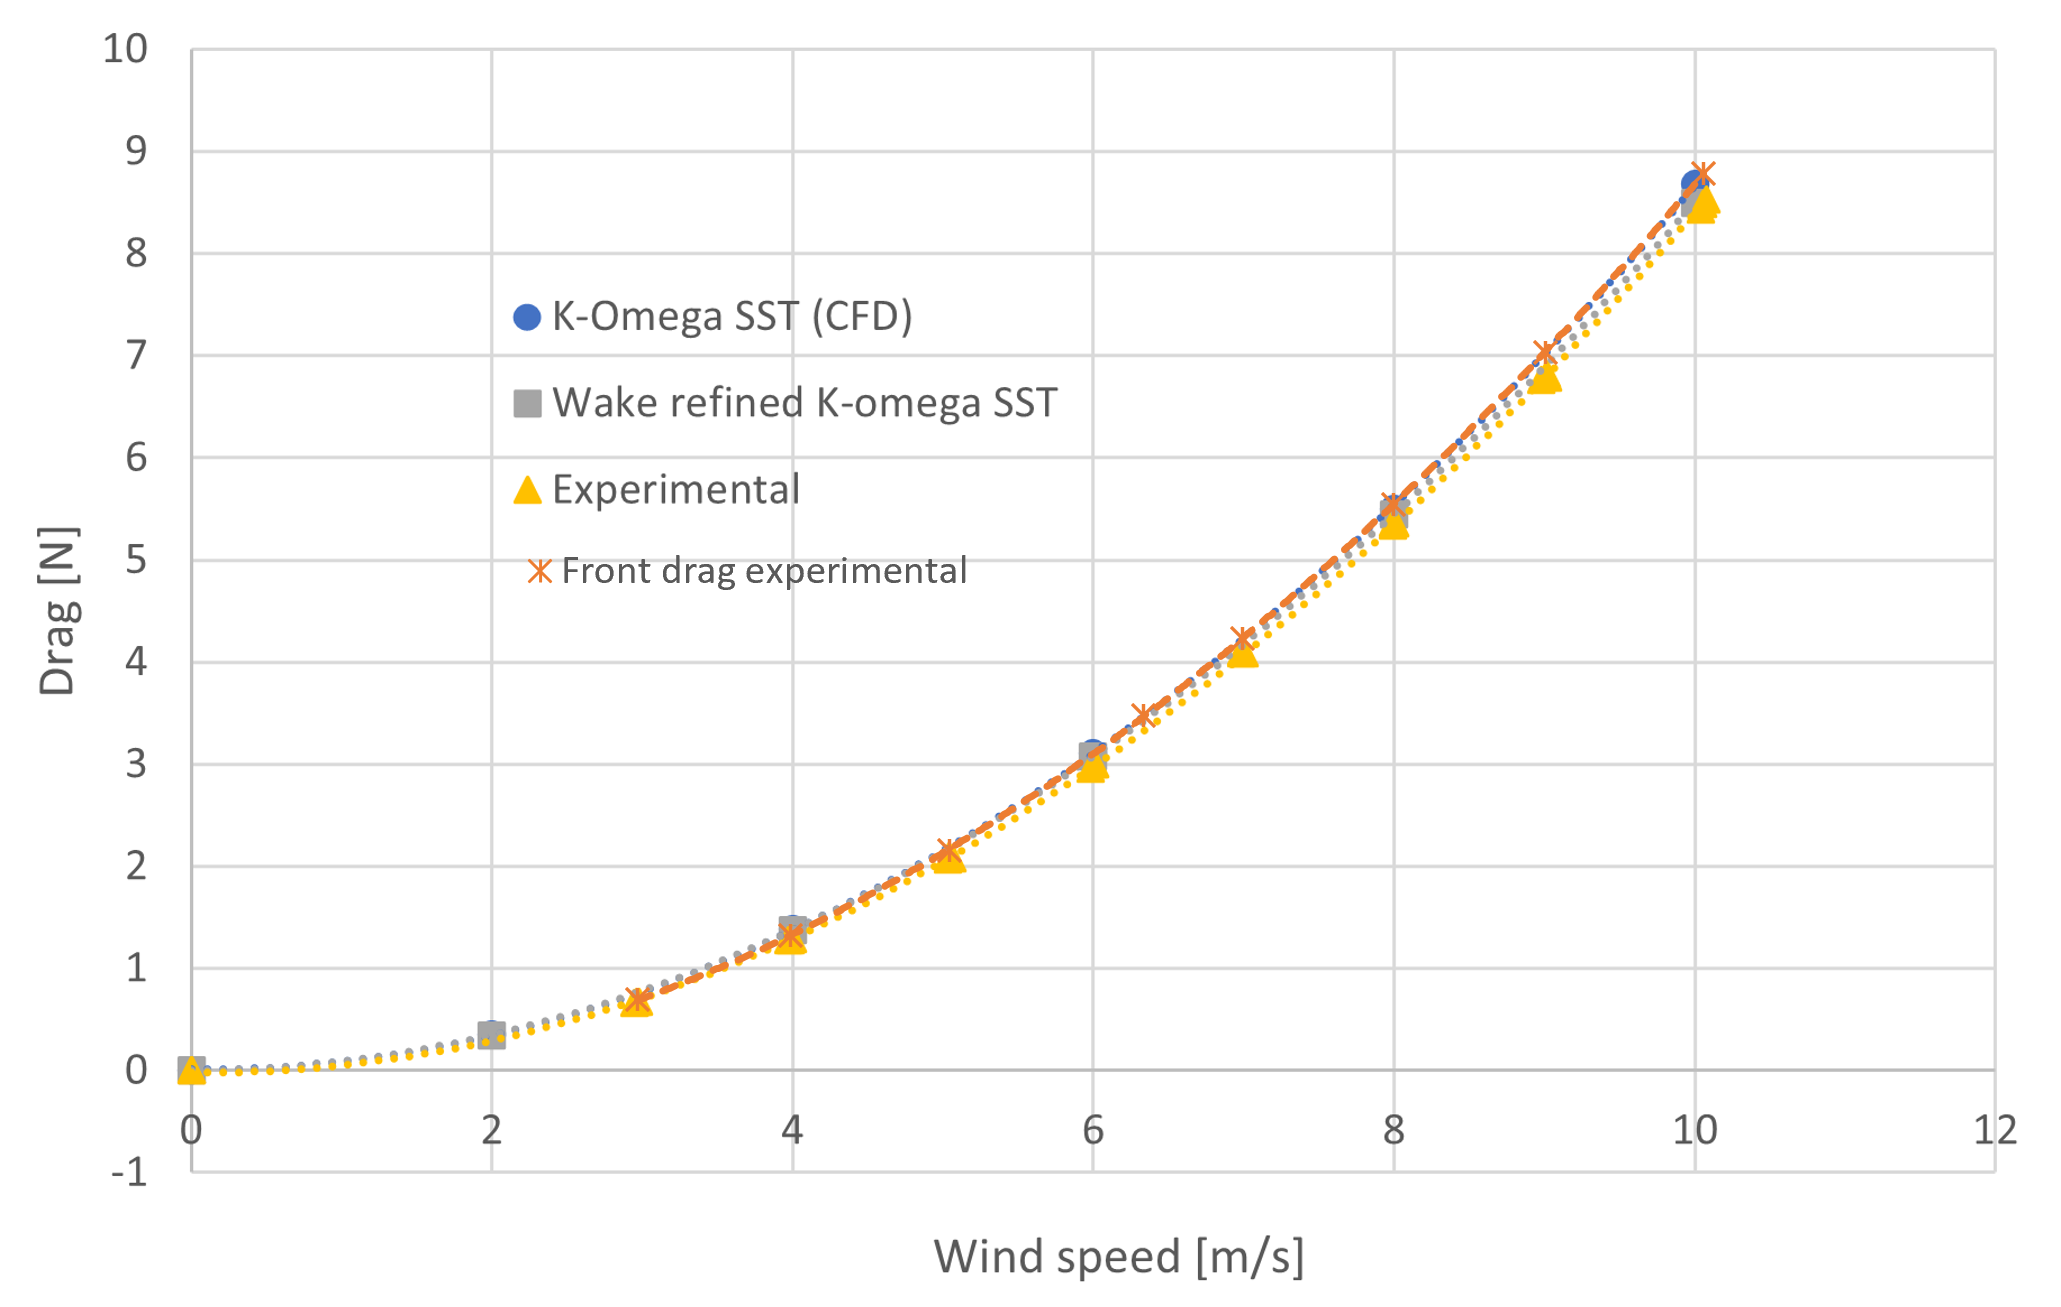
\includegraphics[width=0.75\linewidth]{images/part10.1/dragvalues.png}
    \caption{Drag against free-stream wind speed of CFD and experimental results}
    \label{fig:dragwind}
\end{figure}

The discrepancy in the numerical results shown in Figure \ref{fig:d} can be due to a number of factors. One is the use of a wall function for the surface of the model, some areas are below a $Y^+$ value of 30 which causes the simulation to model the near wall area. The real model uses aluminium profile bars as well as treaded tires which is expected to affect the roughness height in certain areas. This means that these areas should not be modelled with near wall effects as It can be a cause of discrepancies in the wall shear stress.

The results of drag of the refined mesh model especially are in close agreement with the experimental results. The discrepancy caused here could be because the model is a lower fidelity model not capturing small details of the vehicle such as the sprockets, holes, A frame fairings, and use of rectangular cross sections instead of aluminium profiles and many other detailed parts of the high fidelity CAD model. Another factor could be that an unstructured mesh was used without a boundary layer mesh. Although $Y^+$ values are mostly within the bounds of the wall function, there are some minor areas where the first cell height goes through the buffer layer region such as the downstream side of each of the wheels where separation has already occurred.

Despite these factors, the CFD data has been shown to closely represent the drag values of the Experimental data. 

The turbulence intensity, is defined as:

\begin{equation}
    I = \frac{u^{'}_i}{u_i}
\end{equation}

Where $u^{'}_i$ are instantaneous velocity fluctuations and $u_i$ is the mean velocity at that position, giving an indication of the nature of the inflow of the propeller which is situated at the rear of the vehicle. It can be seen from Figure \ref{fig:vehicleiso}, the case of an inflow velocity of 10 m/s, that a large portion of the circle that the propeller traces is subject to high turbulence intensity which can significantly impact the performance of the propeller. In particular, the chain tensioner situated between the two struts of the A-frame creates a large wake in the form of a velocity deficit Figure \ref{fig:vehicleisovelo}. The position of this part can be moved downwards towards the axle of the vehicle to remove the adverse effect to the propeller, but in return the larger area of the tensioner required for this would increase the aerodynamic drag on the vehicle, and therefore this decision must be made with care.

From the drag values obtained, it was possible to make theoretical estimations of the speed the vehicle could have reached at a set wind speed in a real-world setting. The aerodynamical drag (Figure \ref{fig:dragwind}) and the total force on the vehicle for the highest pitch case (Figure \ref{fig:synthesis}.4) were computed at a specific vehicle speed which was then iteratively increased or decreased until the forces were balanced. This yielded the following results: in 10 m/s of wind, with configuration (D) - maximum pitch, the vehicle reached 42\% of the wind speed. For the same environment and configuration (C) (no propeller), the prototype reached 36\% of the wind speed. Although this increase is small, it was shown in the results discussion that the vehicle would have performed better at higher speeds.

\subsection{Efficiency parameters}

Due to practical and time constraints, the propeller could not be tested on a test bench. Therefore, as shown from the equations, the efficiency terms could not be computed solely from experimental data. Although it is not possible to validate the numerical prediction of the propeller performance, the results were used to obtain $F_p$ (Figure \ref{fig:thrustvsRPMplot}. This way, the overall efficiency of the vehicle could be calculated.

The highly-loaded air prop limit equation defined in \cite{drela20dead} was used to calculate the overall efficiency of the vehicle. This overall efficiency of the vehicle $\eta_{o, vehicle}$ corresponds to $\eta_g$ timed by $\eta_v$.

\begin{equation}
F_{\text {net }}=F_{p}\left\{1+\left[V R_{p} \eta_{g} \eta_{v}\left(\frac{2 \pi \rho}{F_{p}} \eta_{\text {swirl }}\right)^{1 / 2}-1\right]^{-1}\right\}^{-1}
\label{eq:highlyloaded}
\end{equation}

Making the following substitution for $F_{net}$ (defined in Equation \ref{eq:fnet}):

\begin{equation}
    F_t = F_{net}-F_{rr}
    \label{eq:ftotal}
\end{equation}

Note that here, the total force being positive signifies thrust on the overall vehicle, unlike what was used in the experimental readings. $F_{rr}$ corresponds to the rolling resistance force.

\begin{equation}
F_{t}+F_{r r}=F_{p}\left(1+\left(V R_{p} \eta_{o, v e h i c l e}\left(\frac{2 \pi \rho}{F_{p}} \eta_{s w i r l}\right)^{\frac{1}{2}}-1\right)^{-1}\right)^{-1}
\label{eq:finaleffi}
\end{equation}

Solving Equation \ref{eq:finaleffi} numerically for the vehicle moving at a ground speed of 8 m/s and using the total force acquired on Figure \ref{fig:individualresults}.4, the efficiency $\eta_{o, vehicle}$ is found to be $0.2$. This is quite low although this efficiency is a multiplication of the transmission and the propeller efficiencies.

\begin{figure}[h]
    \centering
    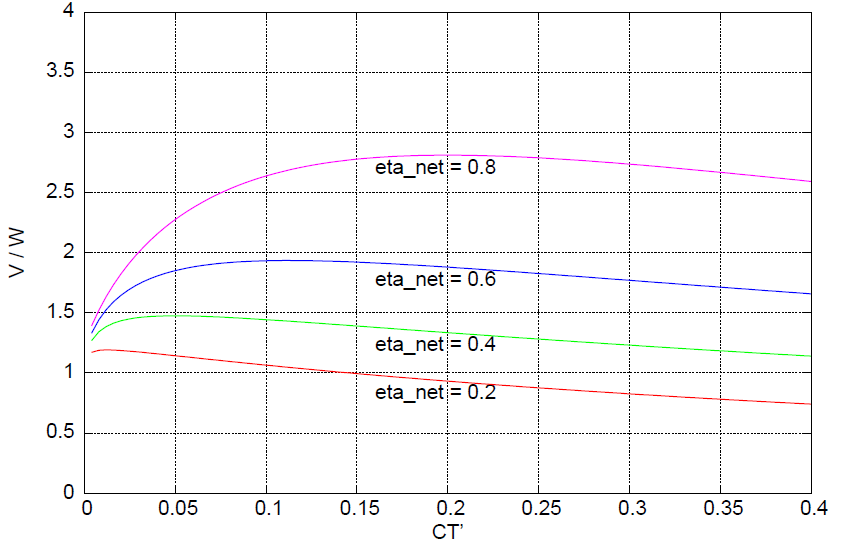
\includegraphics[width=0.65\linewidth]{images/part11/drelaeffi.png}
    \caption{Vehicle/Wind speed ratio for $\eta_{swirl} = 0.95$, $C_r' = 0.02$, $\mathrm{CDA}' = 0.04$ from \cite{drela20dead}}
    \label{fig:drela_effi}
\end{figure}

The "modified air prop thrust coefficient" of the propeller could be computed to be $0.176$ at $8 \mathrm{m/s}$ and for the coarsest pitch. The definition for this coefficient can be found in \cite{drela20dead}. Looking at Figure \ref{fig:drela_effi}, the vehicle would not have been able to reach the speed of the wind. 



